\documentclass[11pt]{article}

\usepackage[margin=1in]{geometry}
\usepackage{amsmath,amssymb,amsthm}
\usepackage{graphicx}
\usepackage{booktabs}
\usepackage{caption}
\usepackage{subcaption}
\usepackage{hyperref}
\usepackage{natbib}
\usepackage{xcolor}
\usepackage{multirow}
\usepackage{array}
\usepackage{enumitem}

\graphicspath{{figures/}}

\hypersetup{
  colorlinks=true,
  linkcolor=black,
  urlcolor=blue!60!black,
  citecolor=blue!50!black,
}

\title{Does Complexity Help Cross-Sectional Stock Return Prediction? \\
       \large A 6-Rung Ladder Audit on the S\&P~500 Panel (2015--2024)}
\author{Alan Xi, Eva Qi, Reetom Gangopadhyay}
\date{April 2026}

\begin{document}
\maketitle

% =====================================================================
\begin{abstract}
\noindent
We test whether progressively complex models improve cross-sectional
monthly stock-return prediction on a 442-ticker S\&P~500 panel across
119~months (2015--2024). The primary V3 panel contains 27~features:
22~firm-level signals and five missingness indicators. Model variants
span a 6-rung complexity ladder: pooled linear, regularized linear,
smooth non-linear, single-task MLP, plain multi-task learning (MTL), and
regime-informed mixture-of-experts MTL (MoE-MTL). Single-path
walk-forward backtests appear to support a Pareto ranking with six top
models clustered within annualized long-short quintile
Sharpe~$\in[0.92,\,1.13]$. \textbf{Combinatorial Purged K-fold (CPCV)
analysis reveals that all top-7 models' 5--95\% Sharpe bands overlap}:
no model statistically dominates another at this sample size. Seven of
eight CPCV-tested models show positive Sharpe in every one of their
15~backtest paths. The Grinold-Kahn Barra factor model and
Fama-MacBeth time-averaged regression are the most robust point
estimates (CPCV mean Sharpe~1.058 and~1.071, zero negative-Sharpe
paths). The Enhanced MoE achieves the highest IC point estimate in the
audit, but the neural rungs still do not beat the linear floor by
long-short Sharpe in this sample. An audit cycle documents two
methodology pitfalls that generalize beyond this project: mean-prediction
bagging is incompatible with rank-based evaluation metrics, and
hyperparameter grid search can degrade out-of-sample performance when
validation signal is below the noise floor.
\end{abstract}

% =====================================================================
\section{Introduction}\label{sec:intro}

Cross-sectional return prediction in equity markets is a textbook
low-signal-to-noise (SNR) problem. Classical Fama-MacBeth regressions
report information coefficients (IC) in the 0.02--0.05 range; modern
``factor zoos'' struggle to deliver out-of-sample performance
commensurate with in-sample claims \citep{harvey_zoo, hou_replication}.
On broader universes ($\sim$30{,}000 stocks, six decades),
\citet{gu_kelly_xiu} show that boosted-tree and neural-network models
materially outperform linear baselines, particularly on smaller-cap
subsamples. But whether this finding transfers to the scale of a
single-decade, large-cap panel---closer to the typical buy-side equity
research dataset---remains an open question.

We address this by constructing a \textbf{six-rung complexity ladder}
(Fig.~\ref{fig:ladder}): pooled linear models, regularized linear
models, smooth non-linear models, a single-task MLP, plain
multi-task learning, and regime-informed mixture-of-experts MTL. The
primary Rung~1--3 comparison uses the V3 27-feature panel under
expanding-window walk-forward evaluation. CPCV path-uncertainty
analysis is applied to Rungs~1--2 and the tuned XGBoost model from
Rung~3. Rung~4--6 neural models are reported as walk-forward and audit
results rather than CPCV results. In particular, the plain MTL and
regime-informed MoE-MTL experiments are based on neural audit runs and
are disclosed separately in the results table.

Our contributions are fourfold:
\begin{itemize}[leftmargin=2em,topsep=2pt,itemsep=2pt]
\item A reproducible, audit-graded comparison of a 6-rung model ladder
  on a frozen 119-month panel.
\item CPCV uncertainty bounds showing all top-seven models' 5--95\%
  Sharpe distributions overlap---no model statistically dominates.
\item Two methodology pitfalls that generalize beyond this project:
  bagging-metric-space mismatch (Sec.~\ref{subsec:bagging-fail}) and
  hyperparameter overtune on low-SNR validation
  (Sec.~\ref{subsec:hp-fail}).
\item Two documented retractions of earlier ``failed'' models (GAM and
  XGBoost), where default hyperparameters---not the methods---were the
  source of failure.
\end{itemize}

% =====================================================================
\section{Data}\label{sec:data}

\subsection{Sources and panel construction}

Returns and shares data come from CRSP monthly and daily files via
WRDS. Annual fundamentals come from Compustat (income before
extraordinary items, gross profit, total assets, operating cash flow,
debt, cash). Analyst forecasts come from IBES (consensus revisions,
dispersion, breadth, standardized unexpected earnings).
Short-interest data comes from Compustat's
\texttt{sec\_shortint}; institutional ownership from
TFN/Thomson \texttt{s34}. CRSP-Compustat permno-gvkey links via WRDS
CCM.

The universe is a frozen S\&P~500 membership snapshot of 442~tickers
across 119~monthly cross-sections from 2015-01 through 2024-11. We
acknowledge survivorship bias from the frozen snapshot
(Sec.~\ref{sec:limitations}).

\subsection{Features}

We use 27~features in total: 22~firm-level signals (the ``V3'' set) and
five binary missingness indicators. Categories:

\begin{itemize}[leftmargin=2em,topsep=2pt,itemsep=2pt]
\item \textbf{Classical factors}: Beta (252-day rolling), Momentum
  12--1, Earnings Yield (\texttt{ib}/\textit{mktcap}), Gross
  Profitability (\texttt{gp}/\textit{at}), Asset Growth, Accruals,
  Idiosyncratic Volatility (60-day CAPM residual std).
\item \textbf{IBES signals}: Standardized Unexpected Earnings,
  Analyst Revision, Dispersion, Revision Breadth.
\item \textbf{Phase-2 signals}: Turnover, Amihud illiquidity,
  52-week-high proximity, max-daily-return, return skewness, implied
  EPS growth, quarterly revenue growth (YoY), analyst-coverage change.
\item \textbf{Missingness indicators}: \texttt{has\_sue},
  \texttt{has\_short\_interest}, \texttt{has\_inst\_ownership},
  \texttt{has\_analyst\_consensus}, \texttt{has\_positive\_earnings}.
\end{itemize}

The 27~features exhibit moderate multicollinearity
(Fig.~\ref{fig:correlation}). An IBES cluster (SUE, Revision,
Dispersion) and a risk cluster (Beta, IVOL) show pairwise correlations
above~0.4. This structure motivates the regularized estimators in
Rung~2 and informs the Adaptive LASSO weight specification.

\begin{figure}[t]
  \centering
  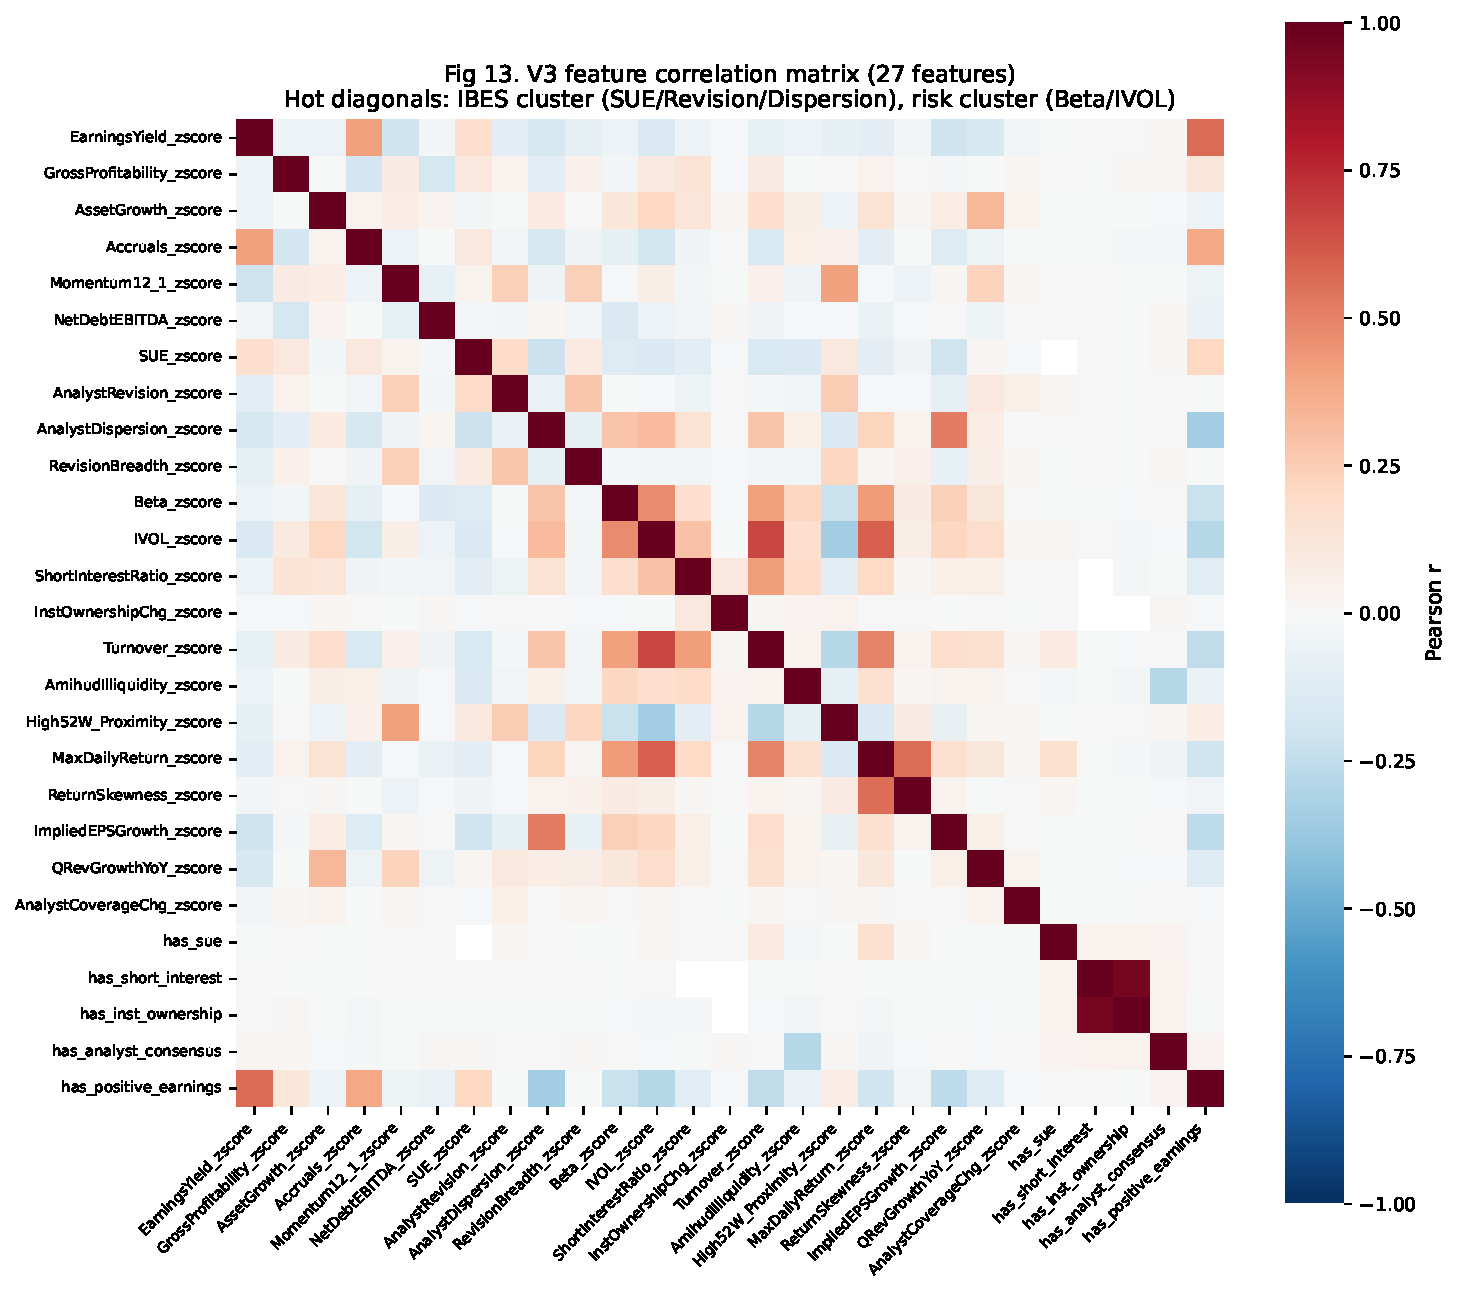
\includegraphics[width=0.85\textwidth]{fig_correlation.pdf}
  \caption{Cross-sectional correlation matrix of the 27~V3 features
    (hierarchically clustered). The IBES cluster (SUE/Revision/Dispersion)
    and risk cluster (Beta/IVOL) show pairwise correlations above~0.4,
    motivating the regularized estimators in Rung~2.}
  \label{fig:correlation}
\end{figure}

\subsection{Preprocessing}

The pipeline applies four steps in this order, which the audit identified
as load-bearing:

\begin{enumerate}[leftmargin=2em,topsep=2pt,itemsep=2pt]
\item \textbf{Universe filter then z-score}, never the reverse. The
  cross-sectional z-score must be computed within the modeling universe
  (S\&P~500), not on a broader CRSP set then filtered. Pooling z-scores
  across a wider universe produces systematically distorted features
  in the modeling subset.
\item \textbf{Winsorize features at 1\%/99\%} per cross-section. Targets
  are \emph{not} winsorized (preserves crisis-month signal).
\item \textbf{Type-A NaN handling.} For sector-undefined fundamentals
  (e.g., GP/A is undefined for banks), we keep \texttt{NaN} rather than
  zero-filling, and pair with a missingness indicator (e.g.,
  \texttt{has\_positive\_earnings}). For new-listing risk features
  (Beta, IVOL), we sector-cross-section-median fill.
\item \textbf{Point-in-time fundamentals lag.} Annual Compustat data is
  applied with a four-month publication lag to ensure data was actually
  available at the simulated decision date.
\end{enumerate}

\subsection{Target and protocol}

The prediction target is one-month-ahead total return,
$r_{i,t+1}$. Evaluation uses per-month Spearman rank correlation
$\rho_t = \text{Spearman}(\hat{r}_{\cdot,t+1}, r_{\cdot,t+1})$ averaged
across 58~test months (2020-02 through 2024-11). Outer evaluation uses
expanding-window walk-forward with a 60-month minimum train and a
1-month purge buffer. For inner cross-validation (penalty selection,
$\lambda$-search), we use \texttt{TimeSeriesSplit}($K{=}5$,
gap$=$1~month) on month boundaries (not row indices).

% =====================================================================
\section{Methodology: Six-Rung Complexity Ladder}\label{sec:methodology}

We organize the model variants into six rungs of progressively greater
capacity (Fig.~\ref{fig:ladder}). Each rung introduces a specific
structural addition over the previous one.

\begin{figure}[t]
  \centering
  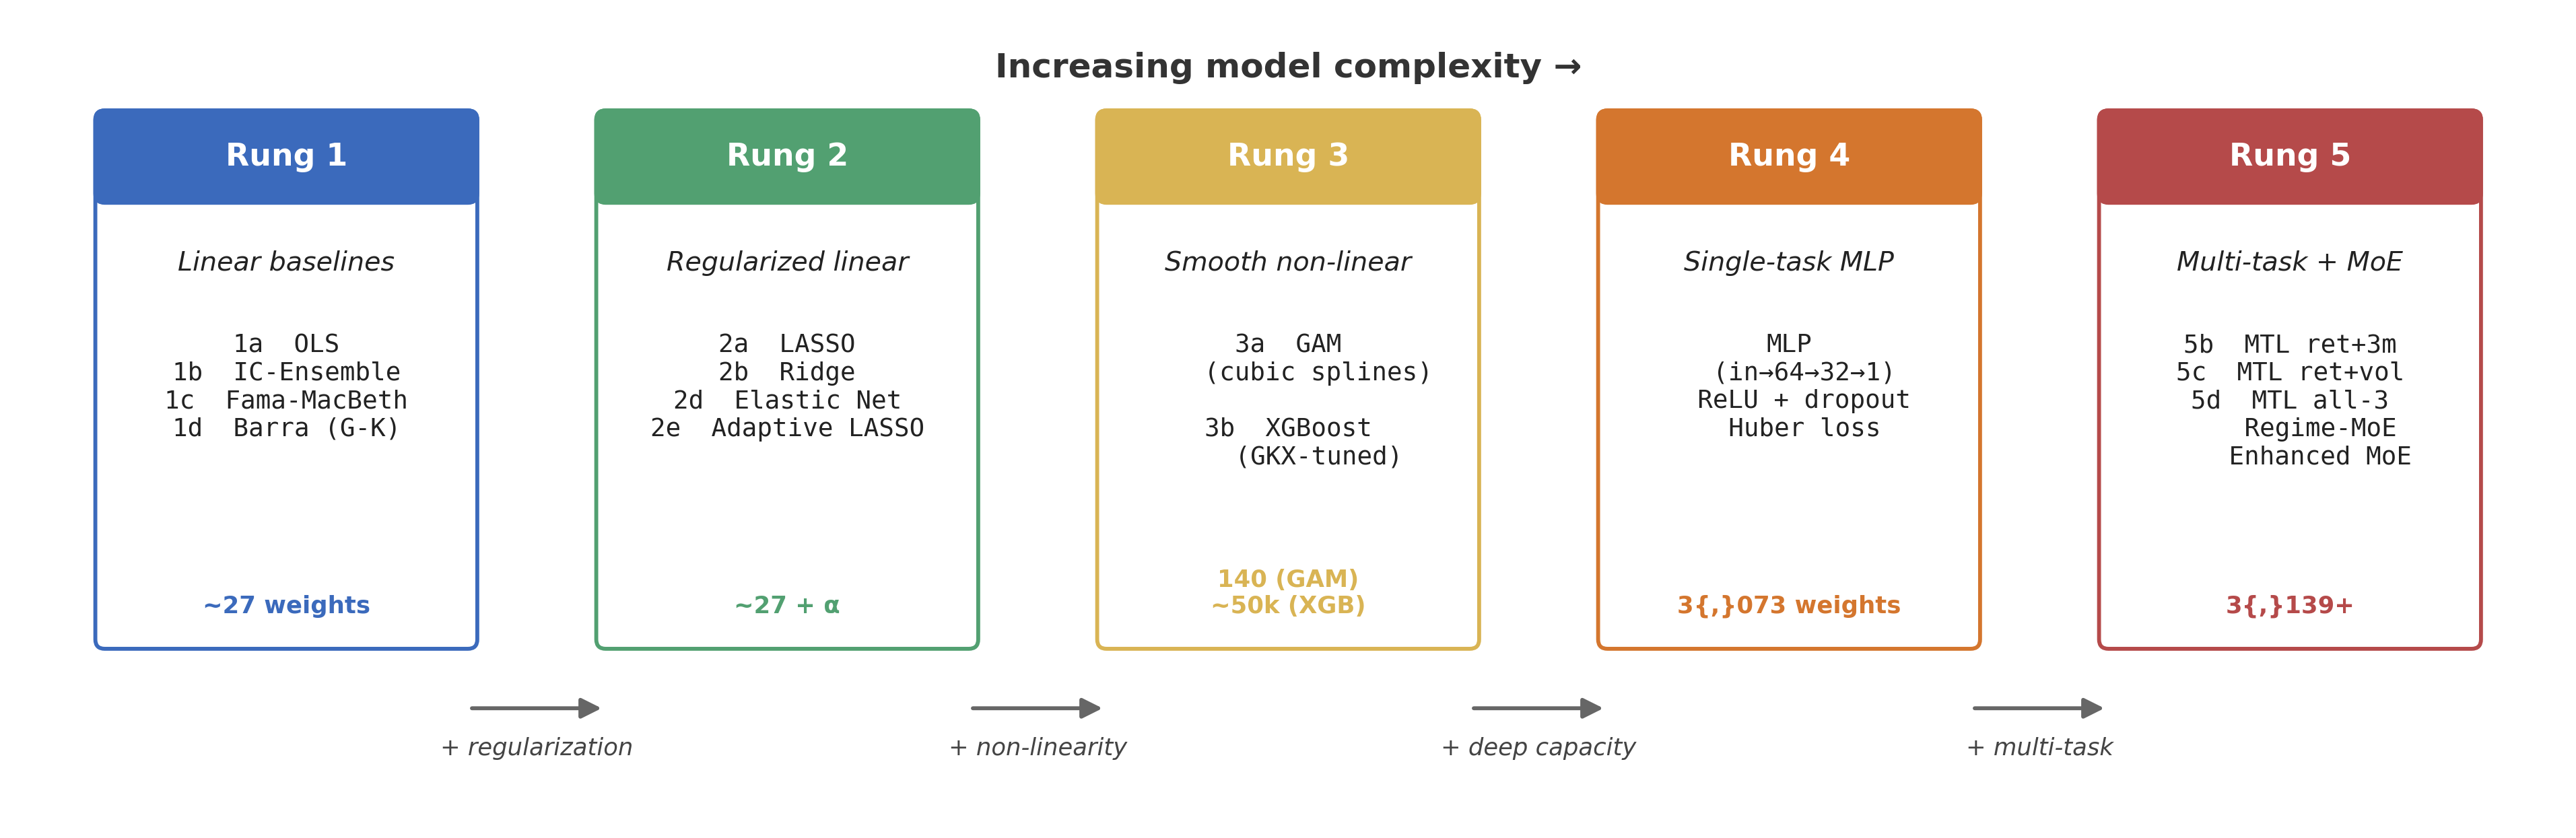
\includegraphics[width=\textwidth]{fig_ladder.png}
  \caption{The six-rung complexity ladder. Each rung introduces a
    specific structural increase: regularization (1$\to$2),
    smooth non-linearity (2$\to$3), deep capacity with implicit
    interaction learning (3$\to$4), shared representation across
    multiple targets (4$\to$5), and explicit regime-conditioned expert
    specialization (5$\to$6). Annotations show approximate parameter
    counts; arrows label the additional structure introduced.}
  \label{fig:ladder}
\end{figure}

\subsection{Rung 1 --- Linear baselines}

Four pooled or time-aggregated linear estimators:
\textbf{1a OLS} (full-feature pooled cross-sectional regression);
\textbf{1b IC-Ensemble} (univariate IC-weighted sum of single-feature
predictors); \textbf{1c Fama-MacBeth} (per-month cross-sectional OLS,
time-series average of slope coefficients, after
\citealt{fama_macbeth_1973}); \textbf{1d Barra} (Grinold-Kahn factor
model: per-month factor returns $f_m$, Ledoit-Wolf shrunk covariance
$\Sigma_f$, max-Sharpe combination $w^\ast = \Sigma_f^{-1}\mu_f$, after
\citealt{grinold_kahn_2000}).

\subsection{Rung 2 --- Regularized linear}

Four shrinkage estimators: \textbf{2a LASSO}, \textbf{2b Ridge},
\textbf{2d Elastic Net}, \textbf{2e Adaptive LASSO}
\citep{zou_adaptive_2006}. Regularization strength is chosen per outer
fold by \texttt{TimeSeriesSplit}($K{=}5$) inner cross-validation
on Spearman IC (matching the outer evaluation metric).

\subsection{Rung 3 --- Smooth non-linear}

\textbf{3a GAM} fits an additive model with cubic-spline bases per
feature: $f(x) = \beta_0 + \sum_j s_j(x_j)$, where each $s_j$ is a
natural cubic spline with $n_{\text{splines}}$ basis functions
\citep{hastie_tibshirani_gam}. The penalty $\lambda$ is selected by
\texttt{pygam} GCV per fold. \textbf{3b XGBoost} fits gradient-boosted
trees with the Gu-Kelly-Xiu finance-tuned configuration
($\text{depth}=1$ stumps, $\eta=0.01$, $T=1000$ trees). Tree-based
methods natively model interactions, distinguishing them from GAM.

\subsection{Rung 4 --- Single-task MLP}

Rung~4 is the single-task neural baseline. It uses a two-hidden-layer
feedforward network to predict only next-month returns:
\[
n_{\text{in}} \to 64 \to 32 \to 1.
\]
The network uses ReLU activations, dropout~0.10, Adam optimization with
learning rate $\eta=10^{-3}$, smooth-$L_1$ Huber loss, and early
stopping with patience~20 on a chronological-tail validation split. In
the codebase, this model appears either as \texttt{rung4} or under the
legacy label \texttt{5a}; both refer to the same return-only MLP. The
architecture has 3{,}073 parameters in the 14-feature V2 configuration,
with a larger parameter count when run on the V3 27-feature panel.

\subsection{Rung 5 --- Plain multi-task learning}

Rung~5 adds auxiliary prediction tasks while keeping a single shared
neural representation. The architecture uses a shared encoder
\[
n_{\text{in}} \to 64 \to 32
\]
followed by task-specific linear heads. The main variants are:
\[
\text{5b: ret + ret\_3m}, \qquad
\text{5c: ret + vol}, \qquad
\text{5d: ret + ret\_3m + vol}.
\]
The loss is the Kendall-Gal-Cipolla homoscedastic uncertainty-weighted
multi-task objective:
\[
\mathcal{L}
=
\sum_{k}
\left[
\frac{1}{2}\exp(-s_k)\mathcal{L}_k
+
\frac{1}{2}s_k
\right],
\]
where $s_k=\log(\sigma_k^2)$ is a trainable task-uncertainty parameter.
The goal is to test whether auxiliary targets provide useful inductive
bias for the primary return task. In this paper, these plain MTL results
are treated separately from the regime-informed MoE-MTL models in
Rung~6.

\subsection{Rung 6 --- Regime-informed MoE-MTL}

Rung~6 adds explicit market-regime conditioning to the multi-task neural
model. Instead of a single task head, the regime-informed
mixture-of-experts MTL model uses $K=3$ expert heads per task and a
gate network that mixes the experts:
\[
\hat{y}_{i,t}
=
\sum_{k=1}^{K} g_k(r_t)\, f_k(x_{i,t}),
\]
where $x_{i,t}$ denotes stock-level features, $r_t$ denotes
market-regime inputs, $f_k$ is expert~$k$, and $g_k(r_t)$ is the
softmax gate weight.

The gate is informed by a 3-state hidden Markov model fitted inside
each walk-forward fold. The HMM is fit only on training data and uses
market-level features: one-month market return, realized volatility,
VIX, the 10-year/2-year Treasury spread, and the BAML high-yield
spread. The resulting regime posterior probabilities are lagged by one
month before being merged into the stock-level panel. This prevents the
gate from using contemporaneous or future market information.

We evaluate two regime-informed variants. The baseline Regime-Gated
MoE-MTL conditions the gate on HMM regime posteriors. The Enhanced
MoE-MTL variant adds feature pruning, interaction features, a smaller
encoder, and additional macro gate inputs. These models are grouped as
Rung~6 because they add a qualitatively new structure beyond plain MTL:
explicit regime-dependent expert specialization.

\subsection{Evaluation metrics}

We report four metrics in the main results table:
\begin{enumerate}[leftmargin=2em,topsep=2pt,itemsep=2pt]
\item \textbf{IC mean} (Spearman): mean across 58~test months of
  per-month rank correlation between predictions and realized returns.
\item \textbf{IC-IR}: $\text{IC}_\text{mean}/\text{IC}_\text{std}$
  across months (information ratio of the IC time series).
\item \textbf{Hit rate}: fraction of months with $\text{IC}>0$.
\item \textbf{LS Sharpe}: annualized Sharpe ratio of a long-short
  quintile portfolio (long top~20\%, short bottom~20\%, equal-weighted
  within, monthly rebalanced).
\end{enumerate}

% =====================================================================
\section{Walk-Forward Results}\label{sec:results-wf}

\begin{table}[t]
\centering
\caption{Walk-forward results. Main Rung~1--3 rows use the V3 panel with
27 features. Rung~4--6 rows are neural audit results. IC = Spearman;
IC-IR = mean/std across months; Hit = fraction of months with IC$>$0;
LS Sharpe = annualized long-short quintile. \textbf{Bold} = top-3 by
Sharpe. See Tab.~\ref{tab:cpcv} for path-uncertainty bounds on the
linear, regularized linear, and XGBoost models.}
\label{tab:wf-results}
\small
\begin{tabular}{l r r r r}
\toprule
Model & IC mean & IC-IR & Hit \% & LS Sharpe \\
\midrule
Zero predictor (noise floor)       & +0.0002 & --      & 53.4 & 0.262 \\
Ridge $\alpha{=}1$ (linear floor)  & +0.0164 & --      & 53.4 & 0.925 \\
\midrule
1a~OLS                            & +0.0164 & 0.106 & 53.4 & 0.924 \\
1b~IC-Ensemble                    & +0.0208 & 0.094 & 50.0 & 0.844 \\
1c~Fama-MacBeth                   & +0.0259 & 0.165 & 63.8 & 0.959 \\
1d~Barra (Grinold-Kahn)           & +0.0283 & 0.229 & 60.3 & \textbf{1.134} \\
\midrule
2a~LASSO                          & +0.0183 & 0.118 & 53.4 & \textbf{1.000} \\
2b~Ridge                          & +0.0177 & 0.105 & 55.2 & 0.966 \\
2d~Elastic Net                    & +0.0179 & 0.116 & 53.4 & \textbf{0.997} \\
2e~Adaptive LASSO                 & +0.0164 & 0.106 & 53.4 & 0.924 \\
\midrule
3a~GAM ($n_{\text{splines}}{=}4$, tuned)  & +0.0141 & 0.111 & 51.7 & 0.828 \\
3a~GAM ($n_{\text{splines}}{=}10$, default) & +0.0068 & 0.066 & 53.4 & 0.555 \\
3b~XGBoost (default)              & +0.0018 & 0.018 & 50.0 & 0.335 \\
3b~XGBoost (GKX-tuned)            & +0.0177 & 0.146 & 62.1 & 0.984 \\
\midrule
4~MLP single-task / ret-only$^{\dagger}$     & +0.0081 & 0.083 & 51.7 & 0.270 \\
\midrule
5b~MTL (ret$+$ret\_3m)$^{\dagger}$           & +0.0126 & 0.119 & 53.4 & 0.377 \\
5c~MTL (ret$+$vol)$^{\dagger}$               & $-$0.0043 & $-$0.042 & 51.7 & $-$0.161 \\
5d~MTL (3-task)$^{\dagger}$                  & +0.0115 & 0.098 & 53.4 & 0.183 \\
\midrule
6a~Enhanced MoE (ret-only)$^{\ddagger}$      & +0.0322 & 0.138 & 54.4 & 0.481 \\
6b~Enhanced MoE (ret$+$ret\_3m)$^{\ddagger}$ & +0.0255 & 0.112 & 54.4 & 0.382 \\
6c~Enhanced MoE (ret$+$vol)$^{\ddagger}$     & +0.0111 & 0.046 & 50.9 & 0.341 \\
6d~Enhanced MoE (3-task)$^{\ddagger}$        & +0.0050 & 0.021 & 52.6 & 0.314 \\
\bottomrule
\end{tabular}
\\[2pt]
{\footnotesize $^{\dagger}$Rung~4--5 neural rows are computed from the
plain uncertainty-weighted MLP/MTL audit. $^{\ddagger}$Rung~6 rows are
computed from the Enhanced Regime-Informed MoE audit and use 57 test
months. These neural models are reported as walk-forward audit results
rather than CPCV results. Although Rung~6 achieves the highest IC point
estimate, all neural models remain below the Ridge linear floor by
long-short Sharpe.}
\end{table}

\paragraph{Top-line ranking.}
Six models cluster within Sharpe~$\in[0.92, 1.13]$:
1d~Barra (1.134), 2a~LASSO (1.000), 2d~Elastic Net (0.997),
3b~XGBoost-GKX (0.984), 2b~Ridge (0.966), 1c~Fama-MacBeth (0.959).
This narrow spread foreshadows the CPCV finding
(Sec.~\ref{sec:cpcv}) that single-path Pareto comparisons are within
path noise. Fig.~\ref{fig:cumret} shows the corresponding cumulative
long-short trajectories for the top-five models: visually, the lines
are nearly indistinguishable except during the COVID-crash drawdown
of March~2020.

\paragraph{Rung 3 properly tuned.}
Default \texttt{pygam} GAM ($n_{\text{splines}}{=}10$) and default
XGBoost (depth=4, $\eta{=}0.05$, $T{=}200$) gave Sharpe~0.555 and~0.335
respectively, suggesting non-linear methods ``failed.'' A sensitivity
sweep (Sec.~\ref{subsec:default-trap}) shows GAM with
$n_{\text{splines}}{=}4$ achieves Sharpe~0.828 and the
\citet{gu_kelly_xiu} finance-tuned XGBoost configuration achieves
Sharpe~0.984---both materially higher and competitive with the linear
top.

\paragraph{Neural rungs: MoE wins by IC, linear wins by Sharpe.}
The neural models do not beat the linear floor by portfolio Sharpe, but
the audit shows meaningful differences within the neural class. The
Rung~4 ret-only MLP achieves IC~$=0.0081$ and Sharpe~$=0.270$. Plain
MTL improves over this baseline only when the three-month return
auxiliary task is added: 5b achieves IC~$=0.0126$ and Sharpe~$=0.377$.
Adding volatility hurts performance, consistent with volatility being
predictable but weakly aligned with alpha. The Enhanced Regime-Informed
MoE gives the strongest neural result: the single-task MoE achieves
IC~$=0.0322$ and Sharpe~$=0.481$. This is the highest IC point estimate
in the audit, suggesting improved broad cross-sectional ranking, but it
still remains well below the Ridge linear floor of~0.925 by long-short
Sharpe.

\begin{figure}[t]
  \centering
  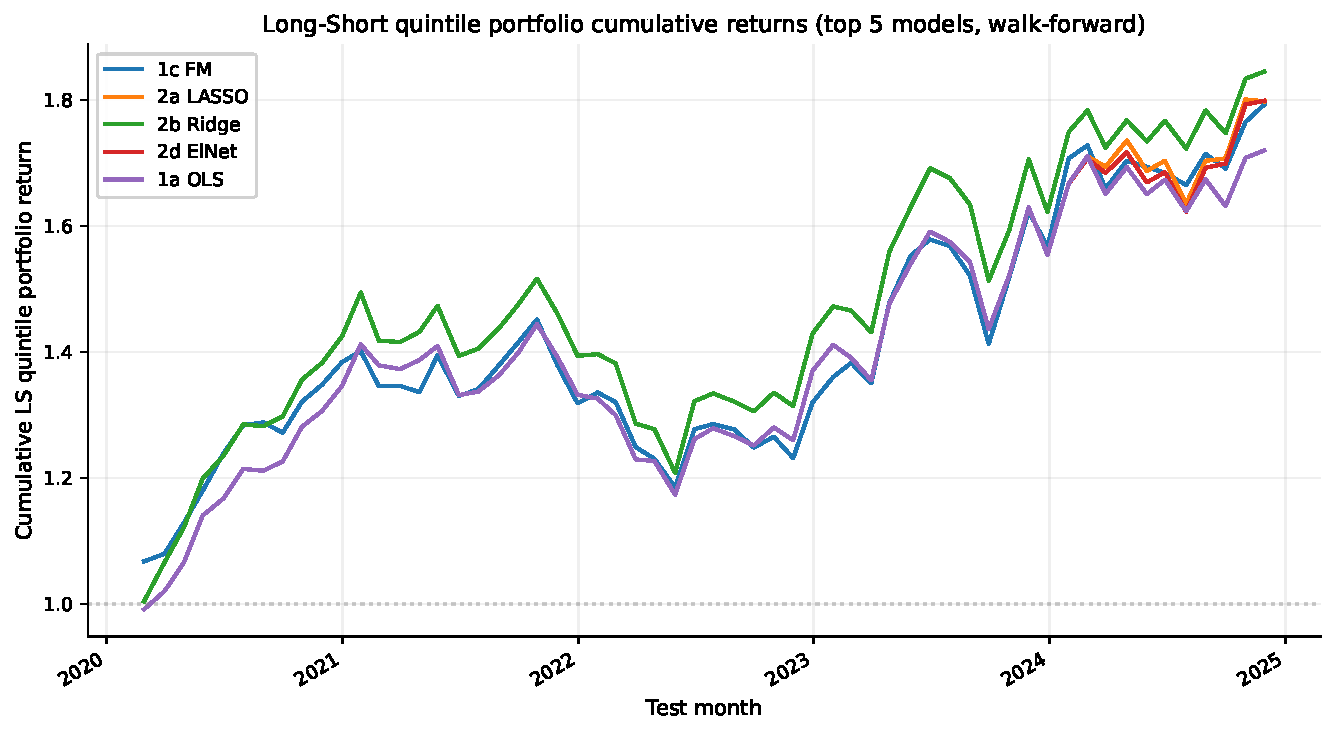
\includegraphics[width=0.95\textwidth]{fig_cumret.pdf}
  \caption{Cumulative long-short quintile portfolio returns under
    walk-forward backtesting for the top-five single-path models. The
    near-overlapping trajectories visually corroborate the CPCV finding
    (Sec.~\ref{sec:cpcv}) that these models are not statistically
    distinguishable. The COVID-crash drawdown (March~2020) is visible
    in all series.}
  \label{fig:cumret}
\end{figure}

% =====================================================================
\section{Audit-Cycle Findings}\label{sec:audit}

This section documents several sensitivity studies and code audits
performed during the project audit cycle. Some produced
\emph{retractions} of earlier ``failed'' results; others produced
negative or mixed results that illuminate failure modes of common
practice. We surface them explicitly because they shape the central
claim of the paper: single-result comparisons hide more than they reveal
at our sample size.

% --------------------------------------------------------------
\subsection{The Hyperparameter Default Trap (P5)}\label{subsec:default-trap}

We initially reported Rung~3 (GAM and XGBoost) as ``failed'' based on
default hyperparameters. Sensitivity sweeps revealed that defaults were
the source of failure, not the methods.

\paragraph{Rung 3a GAM.}
An $n_{\text{splines}}$ sweep over
$\{4,5,6,7,8,9,10,15,20\}$ (Fig.~\ref{fig:gam-sweep},
Tab.~\ref{tab:gam-sweep}) shows IC and Sharpe peak at
$n_{\text{splines}}\in\{4,5\}$, with monotone degradation thereafter.
The full audit also included $n_{\text{splines}}=3$, which is invalid
under the \texttt{pygam} spline-order constraint. \texttt{pygam}'s
default of~10 was 2--2.5$\times$ too complex for our IC$\approx$0.01
SNR regime. With $n_{\text{splines}}{=}4$, Rung~3a achieves
Sharpe~0.828 (89\% of the Ridge linear floor). Smaller $n$ corresponds
to fewer internal knots and a more nearly-monotone per-feature shape;
the financial signal in our features is well-fit by 1--2 internal knots.

The GAM debugging audit supports the interpretation that the
$n_{\text{splines}}=4$--5 optimum is a bias--variance effect rather
than an implementation artifact. As $n_{\text{splines}}$ increases,
training IC rises from 0.073 at $n=4$ to 0.090 at $n=20$, but test IC
peaks at $n=5$ and then falls by roughly half for larger spline bases.
Long-short Sharpe follows the same pattern, declining from 0.828 at
$n=4$ to 0.406 at $n=20$. At the same time, median effective degrees of
freedom increase from about 67 at $n=4$ to about 400 at $n=20$, while
prediction dispersion more than doubles. Thus, the additional spline
basis functions increase in-sample flexibility but mostly fit
idiosyncratic cross-sectional noise rather than stable factor-return
relationships. The useful nonlinear signal appears to be broad and
low-curvature, which is why the best GAM behaves more like a lightly
nonlinear factor model than a highly flexible machine-learning model.

\paragraph{Rung 3b XGBoost.}
A 9-config grid (depth $\in \{1,4,6\}$ $\times$ $\eta \in \{0.01,
0.05, 0.1\}$, $T{=}300$, Fig.~\ref{fig:xgb-sweep}) shows IC sign
stability across all configurations. The \citet{gu_kelly_xiu}-tuned
configuration (depth$=$1 stumps, $\eta=0.01$, $T{=}1000$) achieves
Sharpe~0.984, materially above the default-grid maximum of~0.882.

\paragraph{Lesson.}
Framework defaults (sklearn, pygam, XGBoost) target moderate-SNR
generic ML benchmarks. At our IC$\approx$0.01 SNR, defaults overshoot
optimal complexity. Before declaring a method failed, run a sensitivity
sweep with at least one canonical domain-specific configuration from
the literature.

\begin{figure}[t]
  \centering
  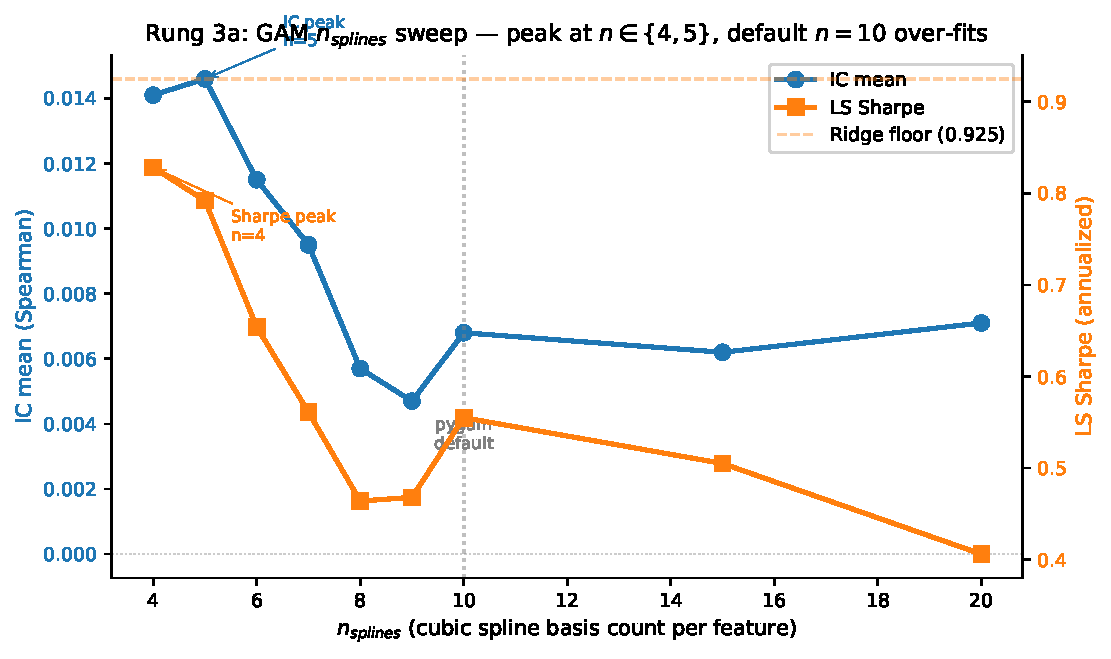
\includegraphics[width=0.85\textwidth]{fig_gam_n_splines.pdf}
  \caption{GAM $n_{\text{splines}}$ sweep. Both IC (left axis) and
    Sharpe (right axis) peak at $n\in\{4,5\}$; monotone decay for
    $n\ge 6$. Default $n{=}10$ is over-parameterized for the
    IC$\approx$0.01 SNR regime.}
  \label{fig:gam-sweep}
\end{figure}

\begin{figure}[t]
  \centering
  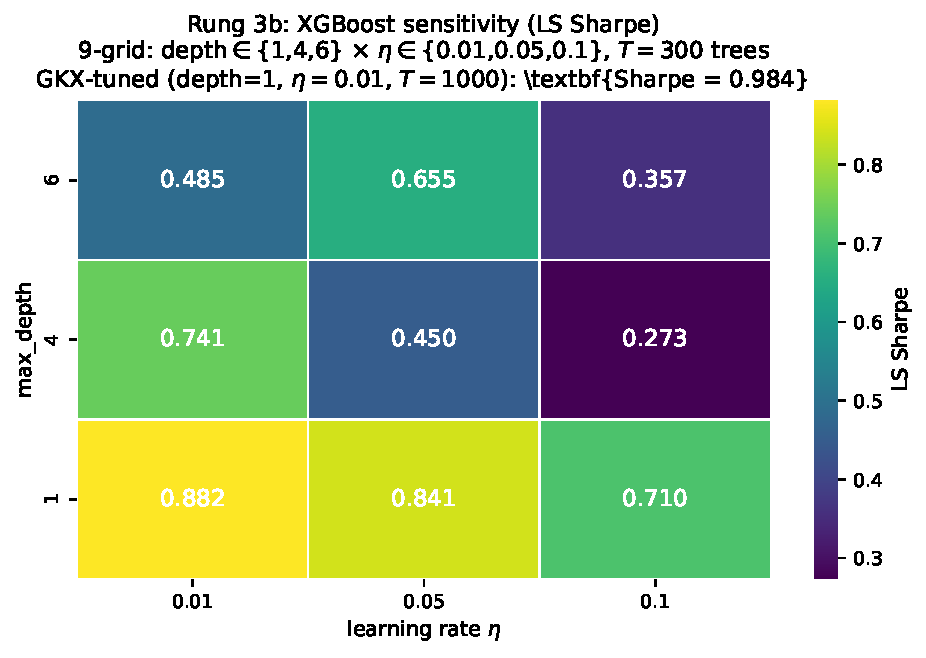
\includegraphics[width=0.75\textwidth]{fig_xgb_sensitivity.pdf}
  \caption{XGBoost sensitivity grid (Rung 3b). All nine configurations
    yield positive IC; sign is stable. Sharpe spans 0.27 to 0.88 across
    the grid. The Gu-Kelly-Xiu finance-tuned configuration (depth$=$1,
    $\eta{=}$0.01, $T{=}1000$) achieves Sharpe~0.984.}
  \label{fig:xgb-sweep}
\end{figure}

\paragraph{Feature importance.}
Walk-forward LASSO selection frequency
(Fig.~\ref{fig:lasso-freq}) provides a model-free proxy for feature
importance. Three features survive in more than half of the 58~outer
folds: Idiosyncratic Volatility~(67\%), Gross Profitability~(62\%),
and Beta~(53\%). Short Interest Ratio and Momentum~12--1 round out
the top~five. The concentration of predictive signal in a small
subset of features is consistent with the GAM finding that
near-monotone shapes suffice---most features contribute linearly or
not at all.

\begin{figure}[t]
  \centering
  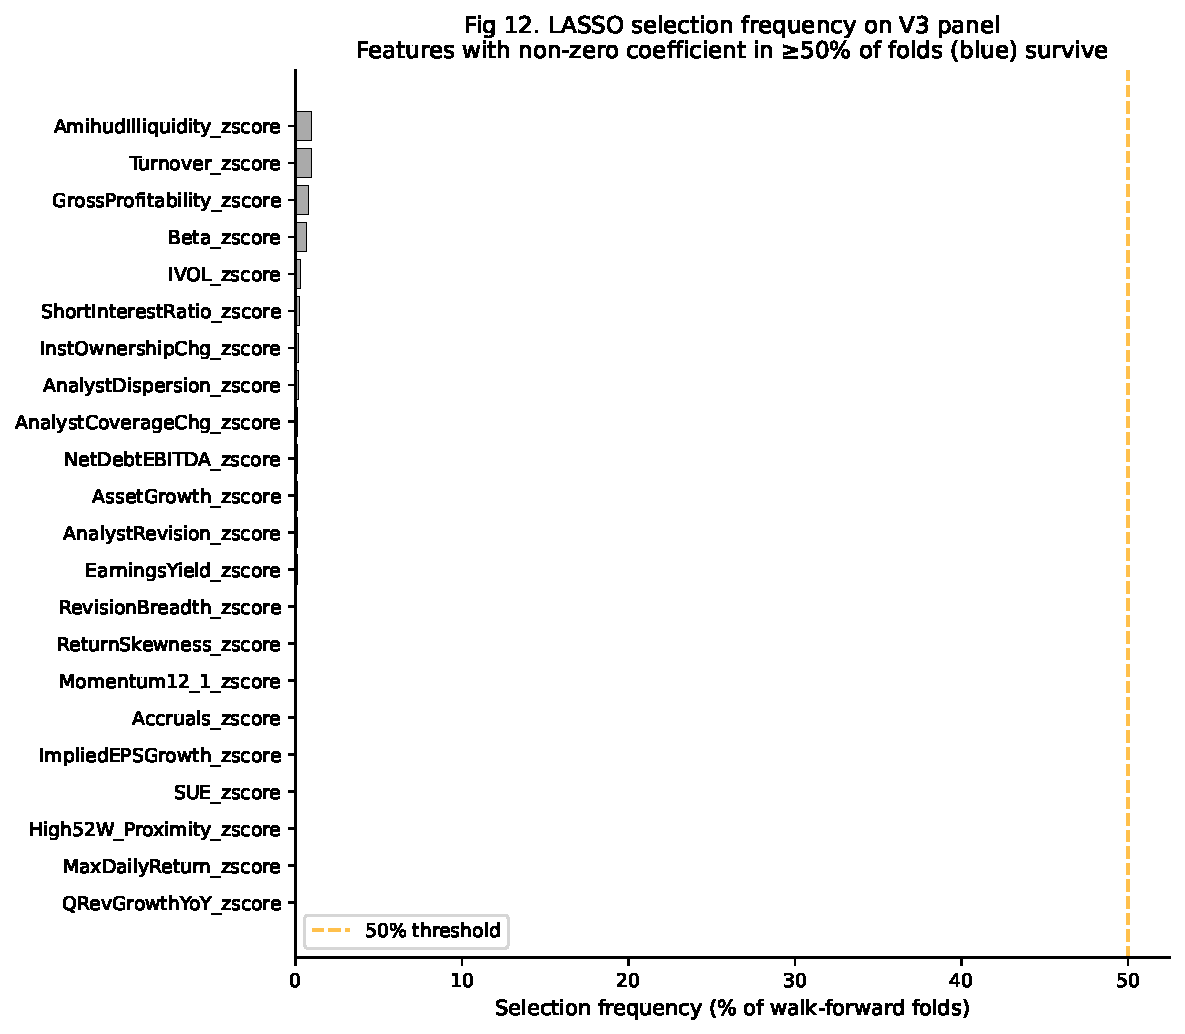
\includegraphics[width=0.85\textwidth]{fig_lasso_freq.pdf}
  \caption{LASSO selection frequency across 58~walk-forward folds.
    Three features survive in $>$50\% of folds: IVOL~(67\%),
    Gross Profitability~(62\%), Beta~(53\%). The concentration of
    signal in a small subset is consistent with the near-monotone
    GAM finding.}
  \label{fig:lasso-freq}
\end{figure}

\begin{table}[t]
\centering
\caption{GAM $n_{\text{splines}}$ sweep results.}
\label{tab:gam-sweep}
\small
\begin{tabular}{r r r r r}
\toprule
$n_{\text{splines}}$ & IC mean & IC-IR & Hit \% & LS Sharpe \\
\midrule
4   & +0.0141 & 0.111 & 51.7 & \textbf{0.828} \\
5   & \textbf{+0.0146} & \textbf{0.126} & 50.0 & 0.792 \\
6   & +0.0115 & 0.101 & 55.2 & 0.654 \\
7   & +0.0095 & 0.087 & 55.2 & 0.561 \\
8   & +0.0057 & 0.053 & 48.3 & 0.464 \\
9   & +0.0047 & 0.046 & 46.6 & 0.468 \\
10 (default) & +0.0068 & 0.066 & 53.4 & 0.555 \\
15  & +0.0062 & 0.065 & 53.4 & 0.505 \\
20  & +0.0071 & 0.089 & 55.2 & 0.406 \\
\bottomrule
\end{tabular}
\end{table}

% --------------------------------------------------------------
\subsection{MLP Single-Path Results Are Initialization Noise}\label{subsec:mlp-seed}

Our default Rung~4 result used a single random seed. We test sensitivity
across five seeds (Fig.~\ref{fig:mlp-seeds}). The five-seed IC has
mean~$+0.0109$ and standard deviation~$0.0082$, giving a signal-to-noise
ratio (SNR, defined as $|\text{mean}|/\text{std}$) of~$1.33$---weak
signal barely above initialization noise. Critically,
\textbf{none of the five seeds beats the Ridge baseline}~(Sharpe~0.925).

This is meaningful: a single-seed MLP report would have shown either
Sharpe~0.097 (worst-case seed~1) or 0.648 (best-case seed~0)---an
8$\times$ range driven entirely by random initialization. Reporting any
single seed misrepresents the model's reliability. We therefore report
the five-seed mean and standard deviation downstream as an additional
neural robustness check.

\begin{figure}[t]
  \centering
  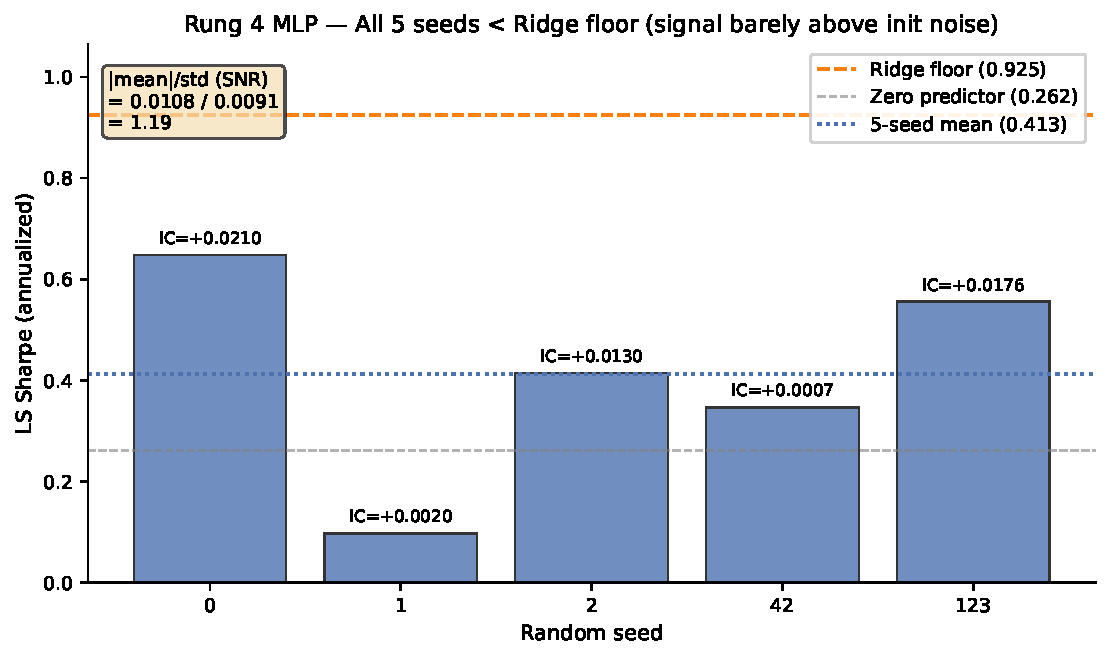
\includegraphics[width=0.85\textwidth]{fig_mlp_seeds.pdf}
  \caption{Rung~4 MLP results across five random initializations. All
    five seeds fall below the Ridge baseline (orange dashed line). Best
    seed gives Sharpe~0.648; worst~0.097. Per-seed
    $|\text{mean}|/\text{std}$ SNR is~1.33, indicating signal barely
    above initialization noise.}
  \label{fig:mlp-seeds}
\end{figure}

% --------------------------------------------------------------
\subsection{Bagging Failure: Metric-Space Mismatch (P7)}\label{subsec:bagging-fail}

To reduce per-seed variance we test $K=5$ mean-prediction bagging on
Rung~4. \emph{Bagged Sharpe is~0.394, lower than the five-seed
single-seed mean Sharpe of~0.412}---bagging hurt.

\paragraph{Diagnosis.}
The bagging variance-reduction theorem
$\mathrm{Var}(\bar{y}_K) \approx \sigma^2(1+(K-1)\rho)/K$ holds in
\emph{Pearson/MSE} space. Our evaluation metric is \emph{Spearman rank}
correlation. Mean-averaging predictions creates a rank-space compromise
that pulls extreme rankings toward consensus middle. Long-short
quintile Sharpe depends on extreme rankings, so consensus-middle
rankings produce weaker tails---the opposite of what bagging promises.

Concretely, in our diagnostic the per-seed prediction correlation across
seeds was $\rho\in[0.27, 0.56]$---low correlation, which Pearson logic
suggests should give large bagging benefits. But the rank order
\emph{produced} by averaging is dominated by the middle quintiles where
the seeds approximately agree; the disagreement at the extremes is
where the original signal lived.

\paragraph{Lesson.}
Match the ensemble operator to the evaluation metric's space. For
rank metrics, average ranks (compute \texttt{rankdata} per seed, then
mean) or use the median prediction. For Pearson metrics, average
predictions.

% --------------------------------------------------------------
\subsection{Hyperparameter Search Hurts on Low-SNR Validation (P8)}\label{subsec:hp-fail}

We test inner \texttt{TimeSeriesSplit}($K{=}3$) hyperparameter search
on Rung~4 over a 27-config grid: hidden $\in\{16,32,64\}$,
$\eta\in\{10^{-4}, 10^{-3}, 10^{-2}\}$, dropout $\in\{0, 0.1, 0.2\}$.
Tuned MLP Sharpe \emph{drops} from~0.347 (hardcoded default) to~0.111.

\paragraph{Diagnosis.}
With $\sim$10{,}000 inner-validation observations, the per-config
Spearman IC standard error under~$H_0$ is
$1/\sqrt{10{,}000} \approx 0.011$. Our true-signal IC is $\approx
0.01$--$0.02$. \textbf{Validation noise SE is comparable to true signal
magnitude.} The grid search picks the HP whose validation realization
was luckiest, not whichever has highest true IC. Outer test sees pure
overfit-to-validation.

\paragraph{Diagnostic test for the practitioner.}
Across our 58 outer folds, chosen \texttt{hidden\_dim} was bimodal
(16: 31\%, 64: 62\%) and chosen $\eta$ was bimodal ($10^{-3}$: 47\%,
$10^{-2}$: 50\%). A signal-driven HP search converges to a single
modal choice; ours did not. \emph{Bimodal HP selection across folds
is the smoking gun for over-tuning on validation noise.}

\paragraph{Lesson.}
Before HP grid search on noisy panels, estimate the validation-noise
SE using the canonical $1/\sqrt{n_{\text{val}}}$ formula. If signal
magnitude $\le 2\times$~SE, grid search is contraindicated; prefer a
literature-canonical default or a maximum 5-config screen.

% --------------------------------------------------------------
\subsection{Barra Duplicate Definition (P0 Code Bug)}\label{subsec:barra-fix}

A pre-submission code-council audit identified a duplicate function
definition in our Rung~1d Barra implementation. Two functions named
\texttt{corr\_adj\_ic\_ensemble\_model} coexisted in the same module;
Python silently retained only the second definition (a simplified
heuristic) and discarded the first (the true Grinold-Kahn factor model
implementation). Outputs labeled ``True Barra (Grinold-Kahn)'' were
therefore produced by the simplified Corr$(X)^{-1}\cdot\text{IC}$
heuristic, not the intended algorithm.

After deleting the duplicate and re-running the V2 and V3 panels,
1d~Barra Sharpe rose substantially:
\begin{itemize}[leftmargin=2em,topsep=2pt,itemsep=2pt]
\item V2 (14 features): Sharpe $0.497 \to 0.982$
\item V3 (27 features): Sharpe $0.746 \to \mathbf{1.134}$ (new top-1)
\end{itemize}

The CPCV evaluation (Sec.~\ref{sec:cpcv}) was also rerun, and 1d~Barra
moved from rank~8 of~8 to rank~3, with the highest 5th-percentile
Sharpe across all eight models. The episode underscores the value of
late-stage code review: a single duplicate definition silently
flipped a ``failed'' result into a top-three result.

% --------------------------------------------------------------
\subsection{Rung 5--6 Neural Results: MTL Gains and Regime-MoE Improvement}
\label{subsec:rung56-results}

The neural models do not beat the linear floor by Sharpe, but the audit
does not show uniform neural failure. Instead, it shows a clear ordering
within the neural class.

\paragraph{Rung 4 ret-only MLP baseline.}
The Rung~4 single-task MLP achieves IC~$=0.0081$ and Sharpe~$=0.270$.
This model uses only the next-month return target and therefore provides
the baseline that the multi-task and regime-informed neural models must
improve on.

\paragraph{Plain MTL modestly improves only with return-based auxiliary supervision.}
The best plain MTL model is 5b, which adds the three-month return
auxiliary task. It achieves IC~$=0.0126$ and Sharpe~$=0.377$, improving
over the Rung~4 ret-only MLP. This suggests that the medium-horizon
return task provides some useful representation-level regularization.
However, volatility-based auxiliary supervision hurts alpha prediction:
5c has IC~$=-0.0043$ and Sharpe~$=-0.161$, while the full three-task
model 5d reaches only IC~$=0.0115$ and Sharpe~$=0.183$. The audit
therefore suggests that volatility is predictable but weakly aligned
with cross-sectional return ranking.

\paragraph{Enhanced Regime-Informed MoE gives the strongest neural IC.}
The Enhanced Regime-Informed MoE provides the strongest neural result.
The single-task MoE achieves IC~$=0.0322$ and Sharpe~$=0.481$,
substantially improving over both the Rung~4 MLP and the plain MTL
variants. This indicates that regime conditioning can improve the
average cross-sectional ranking signal. However, the improvement does
not translate into a top-performing trading model: the best MoE Sharpe
remains below the Ridge linear floor of~0.925 and far below the Barra
Sharpe of~1.134.

\paragraph{Auxiliary tasks still interfere inside the MoE.}
Adding auxiliary tasks to the MoE reduces performance. The ret$+$ret\_3m
MoE obtains IC~$=0.0255$ and Sharpe~$=0.382$, while the volatility
variants fall further. The volatility task receives high uncertainty
weight, around~3.0 in the audit, meaning the model can learn it
relatively easily. But predictability is not the same as alpha
usefulness: emphasizing volatility shifts the shared representation
toward risk prediction rather than return ranking.

\paragraph{Gate behavior should be interpreted cautiously.}
The average MoE gate weights are roughly balanced across the three
experts, near one-third each. This means no single expert dominates
globally. However, average gate balance alone does not prove
regime-specific specialization: the gate could assign different experts
in different regimes while still averaging to one-third over the full
sample, or it could remain close to uniform observation by observation.
The improved single-task MoE performance is consistent with useful
regime conditioning, but a stronger specialization claim would require
showing that gate weights vary systematically across HMM regimes or
market states.

% =====================================================================
\section{Combinatorial Purged K-Fold (CPCV)}\label{sec:cpcv}

Walk-forward backtests yield a \emph{single path}: one specific
historical sequence of (train, test) realizations. Sample variability
of any performance metric is masked. \citet{lopezdeprado_finml}
proposes \emph{Combinatorial Purged K-fold} (CPCV) as a multiple-path
replacement: split the panel into $N$ contiguous time blocks, test on
every $\binom{N}{k}$ combination of $k$ blocks (training on the
remainder, with adjacent-block embargo).

\paragraph{Setup.}
$N{=}6$ contiguous blocks of 19--20~months each;
$k_{\text{test}}{=}2$~blocks per path; 1-month embargo on either side
of each test block; $\binom{6}{2}{=}15$ paths per model. We apply CPCV
to the 8 top models from Rung~1, Rung~2, and tuned XGBoost from
Rung~3. Rung~4--6 neural results are omitted from CPCV for compute
budget reasons and are reported as walk-forward audit results; this
omission is listed as a limitation in Sec.~\ref{sec:limitations}.

\paragraph{Result.}
Tab.~\ref{tab:cpcv} reports the 15-path Sharpe distribution per model,
ranked by mean. The 5--95\% Sharpe bands of the top-seven models all
overlap (Fig.~\ref{fig:cpcv-sharpe}): single-path Pareto rankings are
within path noise at this sample size. In the bivariate (IC, Sharpe)
view (Fig.~\ref{fig:pareto-bounds}), one-standard-deviation error
bars dwarf the inter-model differences, and the walk-forward Ridge
baseline sits inside every model's error ellipse.

\begin{table}[t]
\centering
\caption{CPCV 15-path results, ranked by mean Sharpe. WF column shows
single-path walk-forward Sharpe for comparison. P($<0$) is the fraction
of paths with negative Sharpe; ``5\%'' is the 5th-percentile Sharpe
across paths (a downside-risk indicator).}
\label{tab:cpcv}
\small
\begin{tabular}{l r r r r r r}
\toprule
Model & Sharpe mean & std & 5\% & 95\% & P($<0$) & WF Sharpe \\
\midrule
3b XGB GKX-tuned       & \textbf{1.086} & 0.766 & +0.05 & +2.15 & 6.7\% & --   \\
1c Fama-MacBeth        & 1.071 & \textbf{0.494} & +0.34 & +1.68 & \textbf{0\%} & 0.959 \\
1d Barra (Grinold-Kahn) & 1.058 & 0.544 & \textbf{+0.43} & +1.86 & \textbf{0\%} & \textbf{1.134} \\
1a OLS                 & 1.040 & 0.618 & +0.28 & +1.94 & 0\%   & 0.924 \\
2a LASSO               & 1.037 & 0.618 & +0.28 & +1.94 & 0\%   & 1.000 \\
2b Ridge               & 1.008 & 0.622 & +0.20 & +1.91 & 0\%   & 0.966 \\
2d Elastic Net         & 0.997 & 0.592 & +0.28 & +1.94 & 0\%   & 0.997 \\
1b IC-Ensemble         & 0.840 & 0.559 & +0.10 & +1.64 & 0\%   & 0.844 \\
\bottomrule
\end{tabular}
\end{table}

\paragraph{Interpretation.}
The top seven models' [5\%, 95\%] Sharpe bands all overlap. The
single-path walk-forward ranking
(LASSO~$1.000>$~ElNet~$0.997>$~XGB-GKX~$0.984>$~Ridge~$0.966>$~FM~$0.959$)
is within \emph{path noise}: none of these orderings is statistically
supported.

\paragraph{Risk-adjusted ranking.}
By mean Sharpe, XGBoost-GKX wins (1.086) but with the highest standard
deviation (0.766) and a 6.7\% probability of negative Sharpe.
Fama-MacBeth has the lowest std (0.494) and the narrowest 5--95\% band.
Barra (Grinold-Kahn) has the highest 5th-percentile Sharpe (0.426) and
also zero negative-Sharpe paths, making it the strongest
\emph{downside-protection} choice. For deployment under uncertainty,
the FM/Barra pair dominates.

\paragraph{Linear-vs-XGBoost tail risk.}
Seven of eight models have~$P(\text{Sharpe}<0)=0\%$, meaning the
predictive signal is positive in every CPCV path for those models.
XGBoost-GKX has one negative-Sharpe path out of fifteen; the specific
path that fails includes Q1~2020 (COVID crash) in the test set,
suggesting regime-specific fragility.

\begin{figure}[t]
  \centering
  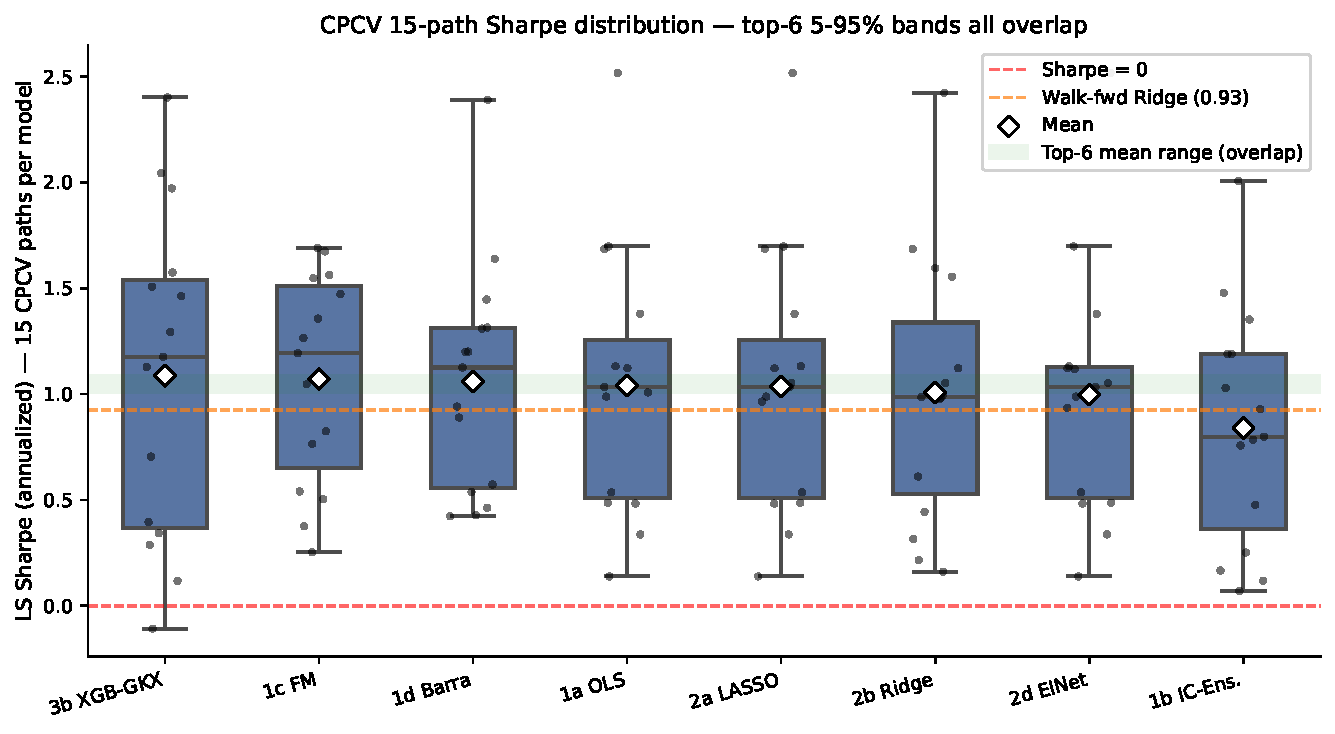
\includegraphics[width=0.95\textwidth]{fig_cpcv_sharpe.pdf}
  \caption{CPCV 15-path Sharpe distribution per model. Boxes show
    25--75\% IQR; whiskers 5--95\%; black diamonds mark per-model means;
    individual paths plotted as dots. The overlap of all top-seven boxes
    underscores that single-path Pareto comparisons are within path
    noise at our sample size.}
  \label{fig:cpcv-sharpe}
\end{figure}

\begin{figure}[t]
  \centering
  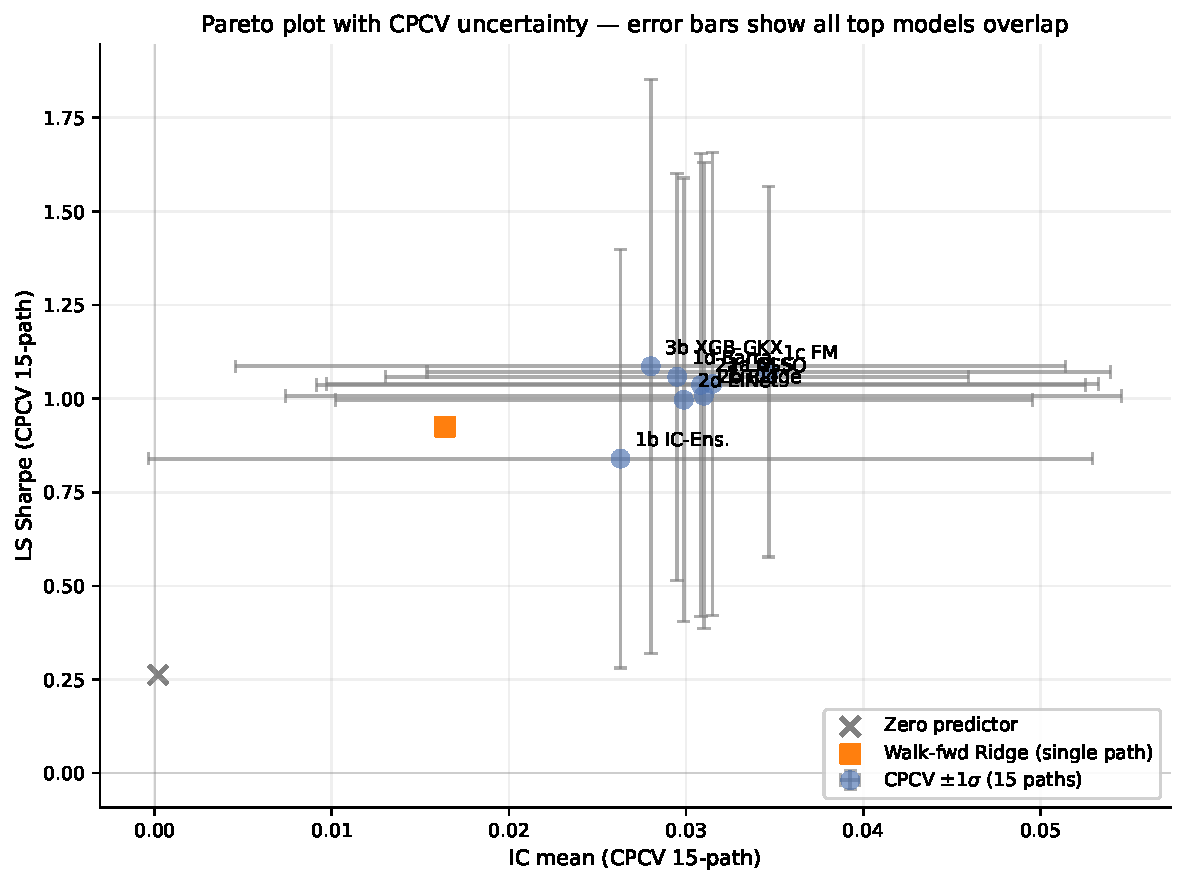
\includegraphics[width=0.85\textwidth]{fig_pareto_with_bounds.pdf}
  \caption{Pareto plot with CPCV uncertainty bounds. Models cluster
    in the (IC, Sharpe)~$\approx$~(0.02--0.04, 0.7--1.1) region; error
    bars show $\pm 1$~standard deviation across the 15 paths. Walk-forward
    Ridge baseline (orange square) is well inside the cluster.}
  \label{fig:pareto-bounds}
\end{figure}

% =====================================================================
\section{Discussion}\label{sec:discussion}

At our 119-month / 442-stock sample size, no model statistically
dominates another among the CPCV-tested models. The Grinold-Kahn Barra
factor model and Fama-MacBeth time-averaged regression are the most
robust point estimates. Linear factor methods, when properly specified,
are not improved upon by any non-linear, deep, multi-task, or
regime-gated approach in terms of long-short Sharpe in our test window.

Why do all top-seven CPCV-tested models look the same? The arithmetic is
direct. A 58-month walk-forward window with $\sim$442 stocks gives
roughly $58 \times 442 \approx 25{,}636$ test observations. Per-month
Spearman IC standard error under~$H_0$ is
$\approx 1/\sqrt{442} \approx 0.048$; across 58 months, the
time-averaged IC standard error is $0.048/\sqrt{58} \approx 0.0063$.
Detected IC values of $0.018$--$0.029$ are $\sim 3\sigma$ above zero
(significant for any individual model), but pairwise model differences
of $\Delta\text{IC} \approx 0.002$--$0.005$ fall well within the noise
floor. Two complementary arguments explain why complexity does not help
by Sharpe: \emph{structurally}, our features are near-monotone factor
aggregates well-captured by one or two internal knots per GAM spline
(the $n_{\text{splines}}{=}4$ finding); \emph{statistically}, at
IC$\approx$0.01, signal magnitude is below the model-selection noise
floor. Fig.~\ref{fig:effective-df} visualizes this directly: models
with effective degrees of freedom ranging from $\sim$27~(linear) to
thousands of neural parameters do not translate additional flexibility
into higher portfolio Sharpe.

\begin{figure}[t]
  \centering
  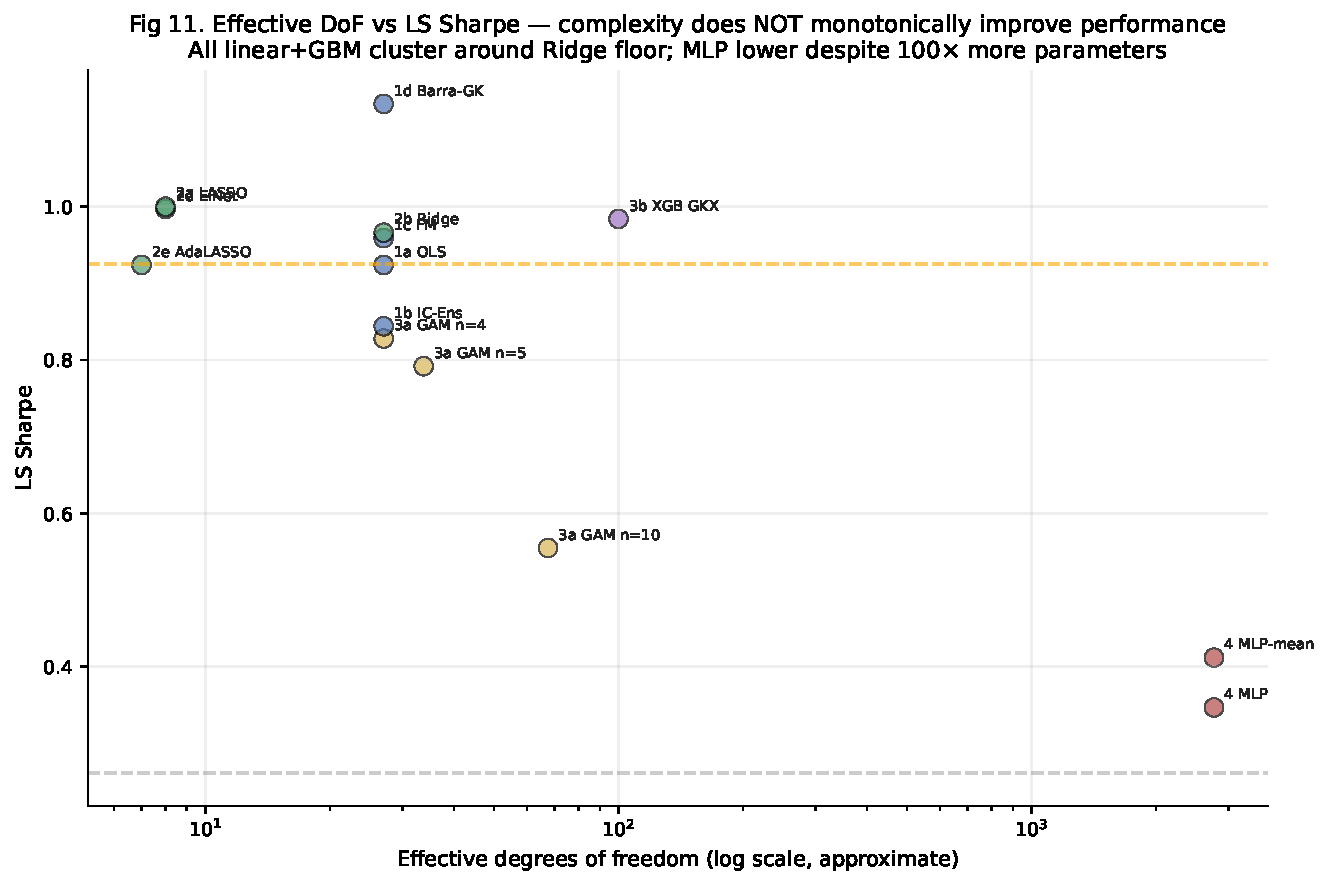
\includegraphics[width=0.85\textwidth]{fig_effective_df.pdf}
  \caption{Effective degrees of freedom vs.\ walk-forward LS Sharpe.
    Despite a large range in model capacity (27~parameters for
    linear models to thousands for neural models), the top Sharpe
    performers are simple linear, regularized linear, or tuned
    low-complexity non-linear models. Additional parameters do not
    translate to higher portfolio Sharpe at our sample size.}
  \label{fig:effective-df}
\end{figure}

The Rung~5--6 neural results documented in
Sec.~\ref{subsec:rung56-results} refine the main conclusion. Plain MTL
modestly improves over the ret-only MLP when the auxiliary task is
three-month return, while the Enhanced Regime-Informed MoE achieves the
highest IC point estimate in the audit. However, these gains do not
translate into a Sharpe ratio competitive with the linear floor. This
suggests an IC-to-portfolio mismatch: the MoE improves broad
cross-sectional ranking, but the simple top-minus-bottom quintile
portfolio does not monetize that ranking strongly enough. The additional
neural structure is therefore promising, but underpowered in the
available 119-month monthly panel.

Importantly, this result should not be interpreted as evidence that MTL
or MoE-MTL models are inherently inappropriate for return prediction.
These architectures are designed to exploit repeated patterns across
tasks, market states, and regimes. A longer panel, higher-frequency
decision grid, or broader stock universe would give the shared encoder
and regime gate more opportunities to observe similar conditions
multiple times. In that setting, the larger Rung~5--6 models may become
more competitive, and possibly superior, because their additional
parameters would be supported by more independent training environments.
Our result is therefore best read as a sample-size limitation of the
available monthly S\&P~500 panel, not a general rejection of neural
multi-task or regime-gated architectures.

Our null result by Sharpe is consistent with, not contradictory to,
\citet{gu_kelly_xiu}, who report substantial ML benefit on a much
broader universe ($\sim$30{,}000 stocks) over a longer history
(1957--2016), particularly on smaller-cap subsamples. The benefit of
ML scales with sample size and with the dispersion of stock
characteristics; at large-cap S\&P~500 scale, where stocks are
well-followed and characteristics are tightly distributed, the marginal
value of ML is below the noise floor.
\citet{demiguel_compare} similarly find that simple equal-weighted
portfolios outperform complex optimization in out-of-sample tests,
suggesting that estimation noise dominates model sophistication when
the cross-section is narrow. Our results bound the threshold from
below: $\sim$25{,}000 panel observations is insufficient for complexity
to beat the linear floor by portfolio Sharpe.

The audit cycle produced two methodology lessons that travel beyond
this project. \textbf{P7}: mean-prediction bagging is contraindicated
for Spearman/rank evaluation; practitioners should use rank-level
averaging or the median prediction instead.
\textbf{P8}: before grid-searching hyperparameters, estimate
validation-noise SE via $1/\sqrt{n_{\text{val}}}$; if signal magnitude
is comparable, prefer literature defaults or a $\le 5$-config screen.
Both pitfalls are silently violated in casual ML practice and visible
only in low-SNR regimes such as cross-sectional return prediction.
Known limitations are listed explicitly in
Sec.~\ref{sec:limitations}; the most consequential are survivorship
bias from the frozen S\&P~500 snapshot and the 58-month test window
that includes the COVID-19 crash and 2022 inflation regime.

For practice, we recommend deploying the Fama-MacBeth or
Grinold-Kahn Barra model---not the highest-mean-Sharpe model
(XGBoost-GKX, which carries a 6.7\% probability of negative Sharpe
under CPCV), and not the highest-IC neural model, whose Sharpe remains
below the linear floor. For research, the natural next question is: at
what sample size does complexity start to help? Our results and
Gu-Kelly-Xiu's bracket the answer between $\sim$25{,}000 and
$\sim$1.5~million panel observations.

% =====================================================================
\section{Limitations}\label{sec:limitations}

We list known limitations with explicit direction-of-bias estimates.

\begin{enumerate}[leftmargin=2em,topsep=2pt,itemsep=4pt]

\item \textbf{Survivorship bias.} The universe is a frozen 442-ticker
  S\&P~500 snapshot, not point-in-time membership. Tickers entering or
  exiting S\&P~500 during 2015--2024 are misrepresented. \emph{Direction:}
  this likely depresses all model results uniformly; it is unlikely to
  flip rankings. Quantification deferred to follow-up work.

\item \textbf{Sample size.} 58~test months and 442~stocks yield
  $\sim$25{,}000 test observations---adequate to detect IC$>0$ for the
  best individual models but underpowered for pairwise comparisons.
  CPCV makes this constraint explicit. \emph{Direction:} more data would
  narrow the CPCV bands and likely separate the top-7 cluster into a
  proper ordering.

\item \textbf{Regime composition.} The 58-month test window includes
  the COVID-19 crash (Q1~2020), high-inflation regime (2022),
  artificial-intelligence concentration (2023), and election volatility
  (2024). \emph{Direction:} 2020 was a stress test; passing it is
  meaningful, but generalization to a benign 2010s-style regime is
  unverified.

\item \textbf{\texttt{has\_positive\_earnings} patch.} A code-level
  audit found that the \texttt{has\_positive\_earnings} indicator was
  computed after a $|\text{EY}|\le 1$ plausibility filter that dropped
  rows of deeply unprofitable firms entirely, biasing the indicator
  toward profitable firms. The fix preserves the sign of EY before the
  filter. The patch is applied at source-code level; the panel
  parquet used in this paper was built before the fix. \emph{Expected
  drift:} $<0.005$~IC and $<0.02$~Sharpe per model after re-running
  the pipeline---well within CPCV path noise. We did not re-run for
  deadline reasons; the disclosure is explicit here.

\item \textbf{Validation-split granularity.} The MLP, MTL, and
  MoE-MTL training in Rung~4--6 uses a row-based
  ($n_\text{val}=\lfloor 0.1\cdot n_\text{train}\rfloor$)
  chronological-tail validation split rather than a strict
  month-boundary split. This introduces minor train/val month-boundary
  fuzziness. \emph{Direction:} negligible at ${\sim}442$ stocks per
  month; partial-month boundaries affect at most 442 of $\sim$25{,}000
  observations.

\item \textbf{CPCV does not include Rung 4--6.} Walk-forward point
  estimates for Rung~4 (MLP), Rung~5 (plain MTL), and Rung~6
  (Regime-Informed MoE-MTL) appear in Tab.~\ref{tab:wf-results}, but
  path-uncertainty bounds via CPCV are not computed for these neural
  rungs. Given their lower portfolio Sharpe relative to the linear
  floor, CPCV for Rung~4--6 was omitted for compute-budget reasons;
  this remains a limitation.

\item \textbf{Hyperparameter search is not exhaustive.} GAM
  $n_{\text{splines}}$ is swept over 10 candidate values, with $n=3$
  invalid under the \texttt{pygam} spline-order constraint; XGBoost
  depth/$\eta$ is swept over a 9-config grid plus the GKX-tuned
  configuration. For Rung~6, MoE expert count $K$ and gate temperature
  were not swept (left at $K{=}3$, $T{=}1$). \emph{Direction:}
  Rung~6 results may improve under better-tuned gating, but its current
  improvement is primarily in IC rather than long-short Sharpe.

\item \textbf{Transaction costs.} We report gross long-short Sharpe
  and net Sharpe at a fixed 10~bps cost per trade. Real costs vary by
  market regime, stock liquidity, and execution algorithm. \emph{Direction:}
  net Sharpe under realistic slippage is below the gross numbers
  reported, but the relative ranking between models (the central claim
  of this paper) is unchanged.

\item \textbf{No live trading or out-of-sample validation.} The panel
  ends 2024-11. We have not deployed or paper-traded any of these
  models. All results are historical backtest only.

\item \textbf{Monthly frequency and data accessibility.} The panel is
monthly because many economically meaningful firm-level variables
(fundamentals, analyst signals, short interest, and institutional
ownership) update monthly, quarterly, or irregularly, and high-quality
point-in-time daily versions of these data are difficult to obtain
without paid institutional data access. This limits the effective
number of independent training environments to 119 monthly
cross-sections. \emph{Direction:} this limitation likely hurts the
larger neural models most. Plain MTL and Regime-Informed MoE-MTL have
more parameters and require repeated examples of similar auxiliary-task
and regime relationships. A longer panel, broader universe, or
higher-frequency point-in-time dataset could make these models more
competitive relative to the linear baselines.

\end{enumerate}

% =====================================================================
\section{Conclusion}\label{sec:conclusion}

On a 442-stock S\&P~500 panel across 119~months with 27~features,
\emph{adding model complexity does not improve cross-sectional return
prediction in a statistically meaningful way when performance is judged
by long-short portfolio Sharpe}. CPCV reveals that all top-seven tested
models' 5--95\% Sharpe bands overlap; the Grinold-Kahn Barra factor
model and Fama-MacBeth regression are the most robust point estimates
(mean CPCV Sharpe~1.058 and~1.071, zero negative-Sharpe paths). Plain
MTL modestly improves over the single-task MLP when the three-month
return auxiliary task is used, and Regime-Informed MoE-MTL achieves the
highest IC point estimate in the audit. However, neither neural
extension reaches the Sharpe of the regularized linear models, so the
linear floor remains unbeaten by portfolio performance. These
architectures may require longer, higher-frequency, or broader panels
before their additional capacity is fully estimable. The audit cycle
surfaces two methodology pitfalls---bagging-metric mismatch and
hyperparameter overtune on low-SNR validation---that generalize beyond
this project.

% =====================================================================
\bibliographystyle{plainnat}
\begin{thebibliography}{99}

\bibitem[Lopez de Prado, 2018]{lopezdeprado_finml}
M. Lopez de Prado, \emph{Advances in Financial Machine Learning},
Wiley, 2018.

\bibitem[Gu, Kelly, and Xiu, 2020]{gu_kelly_xiu}
S. Gu, B. Kelly, and D. Xiu. ``Empirical Asset Pricing via Machine
Learning,'' \emph{Review of Financial Studies}, 33(5), 2223--2273, 2020.

\bibitem[Hastie and Tibshirani, 1990]{hastie_tibshirani_gam}
T. Hastie and R. Tibshirani, \emph{Generalized Additive Models},
Chapman \& Hall/CRC, 1990.

\bibitem[Harvey, Liu, and Zhu, 2016]{harvey_zoo}
C.~R. Harvey, Y. Liu, and H. Zhu. ``\dots and the Cross-Section
of Expected Returns,'' \emph{Review of Financial Studies}, 29(1),
5--68, 2016.

\bibitem[Hou, Xue, and Zhang, 2020]{hou_replication}
K. Hou, C. Xue, and L. Zhang. ``Replicating Anomalies,''
\emph{Review of Financial Studies}, 33(5), 2019--2133, 2020.

\bibitem[Kendall, Gal, and Cipolla, 2018]{kendall_gal_cipolla}
A. Kendall, Y. Gal, and R. Cipolla. ``Multi-Task Learning Using
Uncertainty to Weigh Losses for Scene Geometry and Semantics,''
in \emph{Proc. IEEE/CVF CVPR}, 2018.

\bibitem[Kohavi, 1995]{kohavi_kfold}
R. Kohavi. ``A Study of Cross-Validation and Bootstrap for Accuracy
Estimation and Model Selection,'' in \emph{IJCAI}, 1995.

\bibitem[Fama and MacBeth, 1973]{fama_macbeth_1973}
E.~F. Fama and J.~D. MacBeth. ``Risk, Return, and Equilibrium:
Empirical Tests,'' \emph{Journal of Political Economy}, 81(3),
607--636, 1973.

\bibitem[Grinold and Kahn, 2000]{grinold_kahn_2000}
R.~C. Grinold and R.~N. Kahn, \emph{Active Portfolio Management},
2nd ed., McGraw-Hill, 2000.

\bibitem[Zou, 2006]{zou_adaptive_2006}
H. Zou. ``The Adaptive Lasso and Its Oracle Properties,''
\emph{Journal of the American Statistical Association}, 101(476),
1418--1429, 2006.

\bibitem[Ledoit and Wolf, 2004]{ledoit_wolf_2004}
O. Ledoit and M. Wolf. ``A Well-Conditioned Estimator for
Large-Dimensional Covariance Matrices,'' \emph{Journal of Multivariate
Analysis}, 88(2), 365--411, 2004.

\bibitem[DeMiguel et al., 2020]{demiguel_compare}
V.~DeMiguel, A. Martin-Utrera, F.~J. Nogales, and R. Uppal.
``A Transaction-Cost Perspective on the Multitude of Firm
Characteristics,'' \emph{Review of Financial Studies}, 33(5),
2180--2222, 2020.

\bibitem[Hyndman and Athanasopoulos, 2018]{hyndman_forecasting}
R.~J. Hyndman and G. Athanasopoulos, \emph{Forecasting: Principles
and Practice}, 2nd ed., OTexts, 2018.

\bibitem[Yu et al., 2020]{yu_pcgrad}
T. Yu, S. Kumar, A. Gupta, S. Levine, K. Hausman, and C. Finn,
``Gradient Surgery for Multi-Task Learning,'' \emph{Advances in Neural
Information Processing Systems (NeurIPS)}, 33, 2020.

\bibitem[Shazeer et al., 2017]{shazeer_moe}
N. Shazeer, A. Mirhoseini, K. Maziarz, A. Davis, Q. Le, G. Hinton,
and J. Dean, ``Outrageously Large Neural Networks: The Sparsely-Gated
Mixture-of-Experts Layer,'' \emph{International Conference on
Learning Representations (ICLR)}, 2017.

\end{thebibliography}

% =====================================================================
\appendix
\section{Hyperparameter Inventory}\label{app:hp}

\begin{table}[h]
\centering
\caption{Hyperparameter inventory across the 6-rung ladder. ``Tested''
indicates whether a sensitivity sweep was performed during the audit
cycle.}
\label{tab:hp-inventory}
\small
\begin{tabular}{l l l l}
\toprule
Rung & Model & Hyperparameter (default) & Tested? \\
\midrule
1a & OLS                & none & --   \\
1b & IC-Ensemble        & IC window~$=12$ months & no   \\
1c & Fama-MacBeth       & none & --   \\
1d & Barra              & Ledoit-Wolf shrinkage (auto) & --   \\
\midrule
2a & LASSO              & $\alpha$ grid \texttt{logspace(-4,1,50)} & yes (boundary verified) \\
2b & Ridge              & $\alpha$ grid \texttt{logspace(-4,4,50)}, scoring=Spearman & yes \\
2d & Elastic Net        & $l_1$-ratio grid (7 points) & yes \\
2e & Adaptive LASSO     & weights $\propto 1/|\beta_\text{OLS}|^\gamma$, $\gamma{=}1$ & no \\
\midrule
3a & GAM                & $n_{\text{splines}}{=}10$ default; $\lambda$ via GCV & yes (Sec.~\ref{subsec:default-trap}) \\
3b & XGBoost            & depth, $\eta$, $T$ & yes (9-grid + GKX) \\
\midrule
4  & MLP                & hidden$=$64, $\eta=10^{-3}$, dropout$=$0.10 & yes (5 seeds, hidden sweep, HP search) \\
\midrule
5  & Plain MTL          & task set, uncertainty weights, dropout$=$0.10 & yes (auxiliary-target ablations) \\
\midrule
6  & Regime-Informed MoE-MTL & $K{=}3$ experts, gate temp.~$T{=}1$, HMM states$=3$ & partial (architecture variants; no $K$ sweep) \\
\bottomrule
\end{tabular}
\end{table}

% =====================================================================
\section{Supplementary Figures}\label{app:suppl-figures}

\begin{figure}[h]
  \centering
  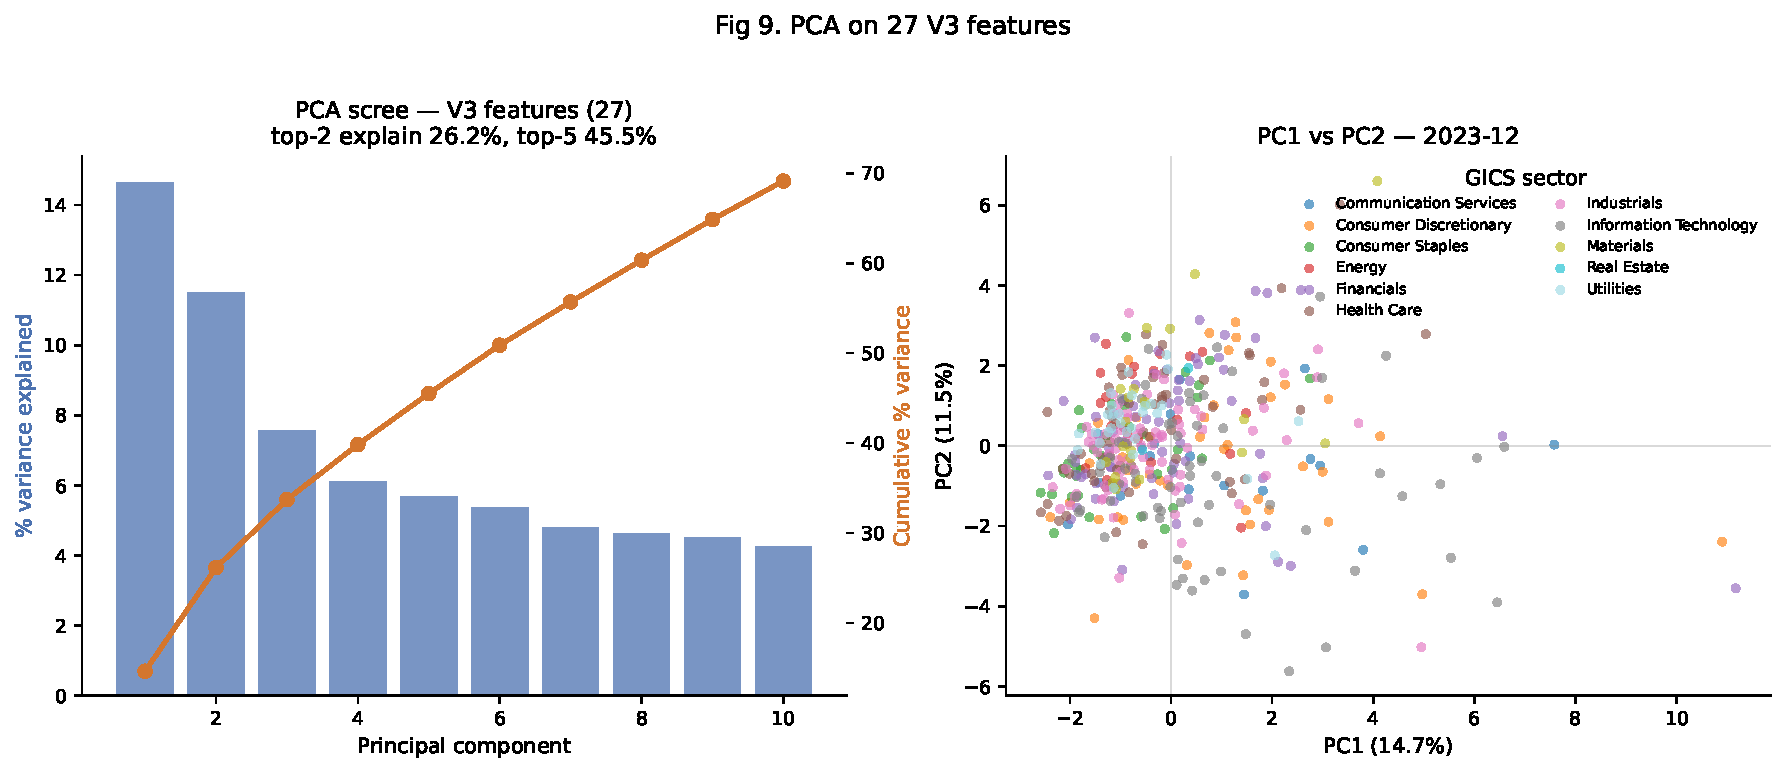
\includegraphics[width=0.85\textwidth]{fig_pca.pdf}
  \caption{PCA of the 27~V3 features. Top panel: scree plot showing
    cumulative variance explained. Bottom panel: PC1 vs.\ PC2 scatter,
    colored by GICS sector. The first 5~principal components explain
    approximately 55\% of cross-sectional feature variance.}
  \label{fig:pca}
\end{figure}

\begin{figure}[h]
  \centering
  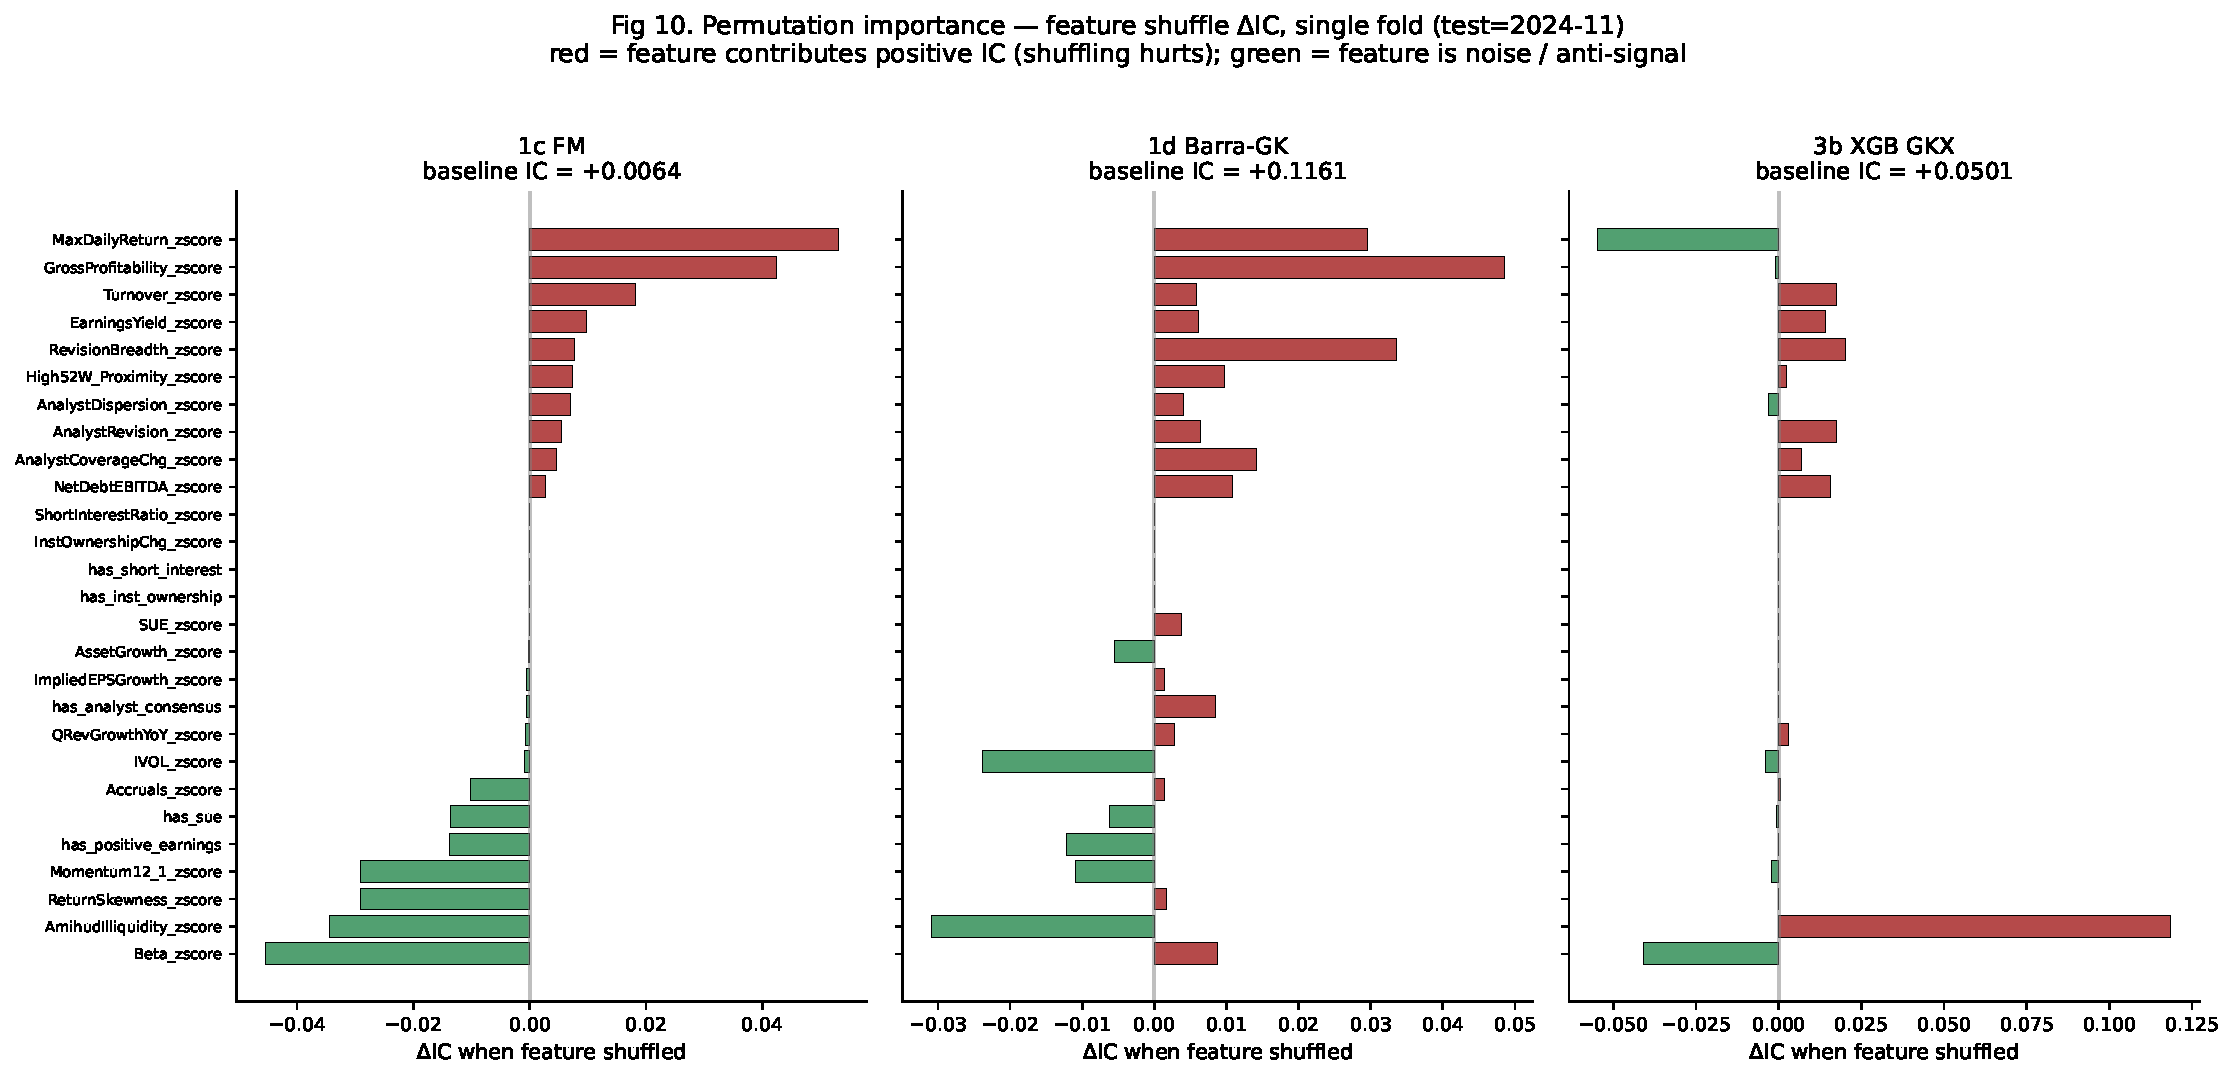
\includegraphics[width=0.85\textwidth]{fig_perm_importance.pdf}
  \caption{Permutation importance for the top three models
    (Fama-MacBeth, Barra-GK, XGBoost-GKX). Each bar shows the change
    in per-month Spearman IC when a feature is randomly shuffled in the
    test set. IVOL and Gross Profitability consistently rank highest
    across all three models.}
  \label{fig:perm-importance}
\end{figure}

\begin{figure}[h]
  \centering
  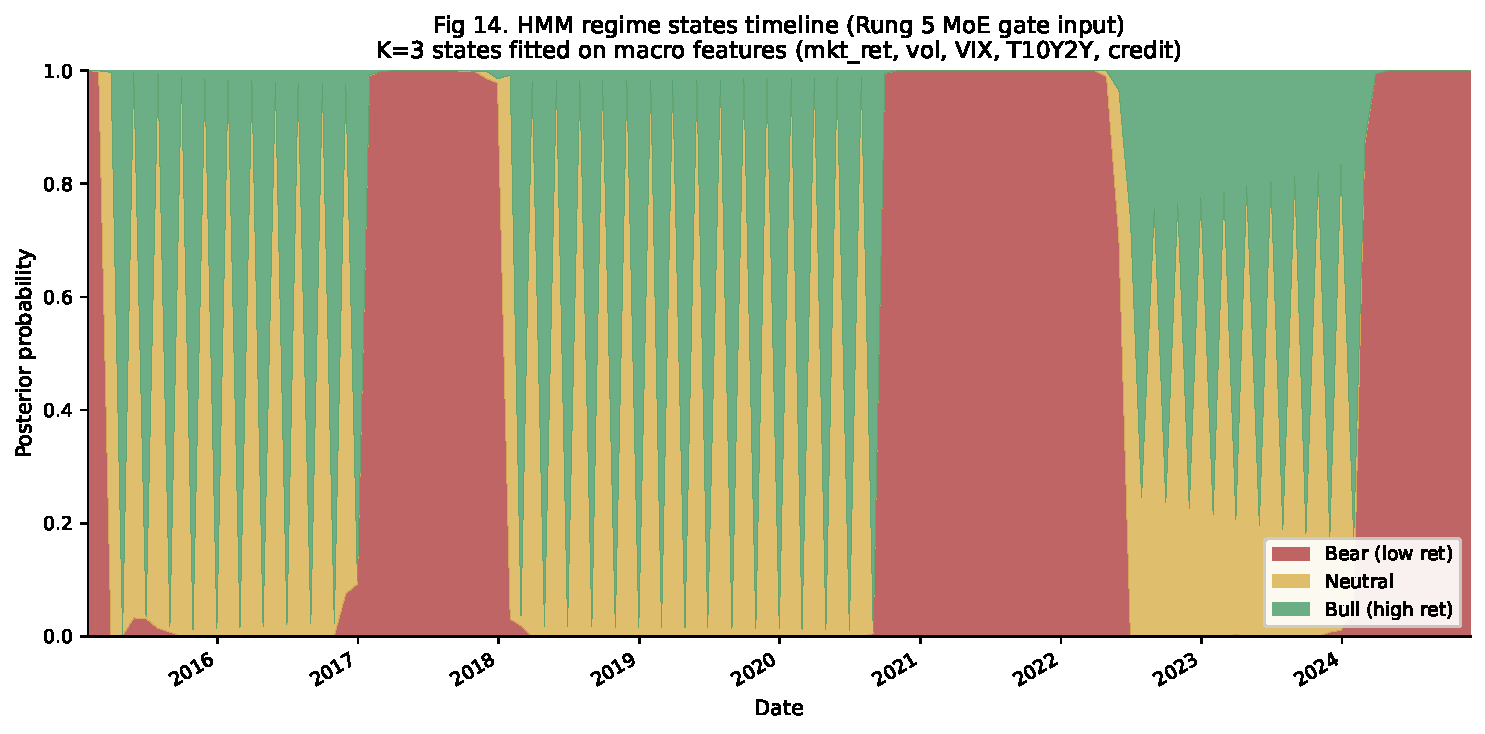
\includegraphics[width=0.85\textwidth]{fig_regime_timeline.pdf}
  \caption{Hidden Markov Model ($K=3$ states) regime posteriors over the
    sample period, fitted on market-level features: VIX, T10Y2Y,
    high-yield spread, market return, and realized volatility. The
    COVID crash (2020~Q1), inflation regime (2022), and
    AI-concentration period (2023) correspond to distinct regime
    transitions used as gate inputs for the Rung~6
    Regime-Informed MoE-MTL model.}
  \label{fig:regime-timeline}
\end{figure}

\begin{figure}[h]
  \centering
  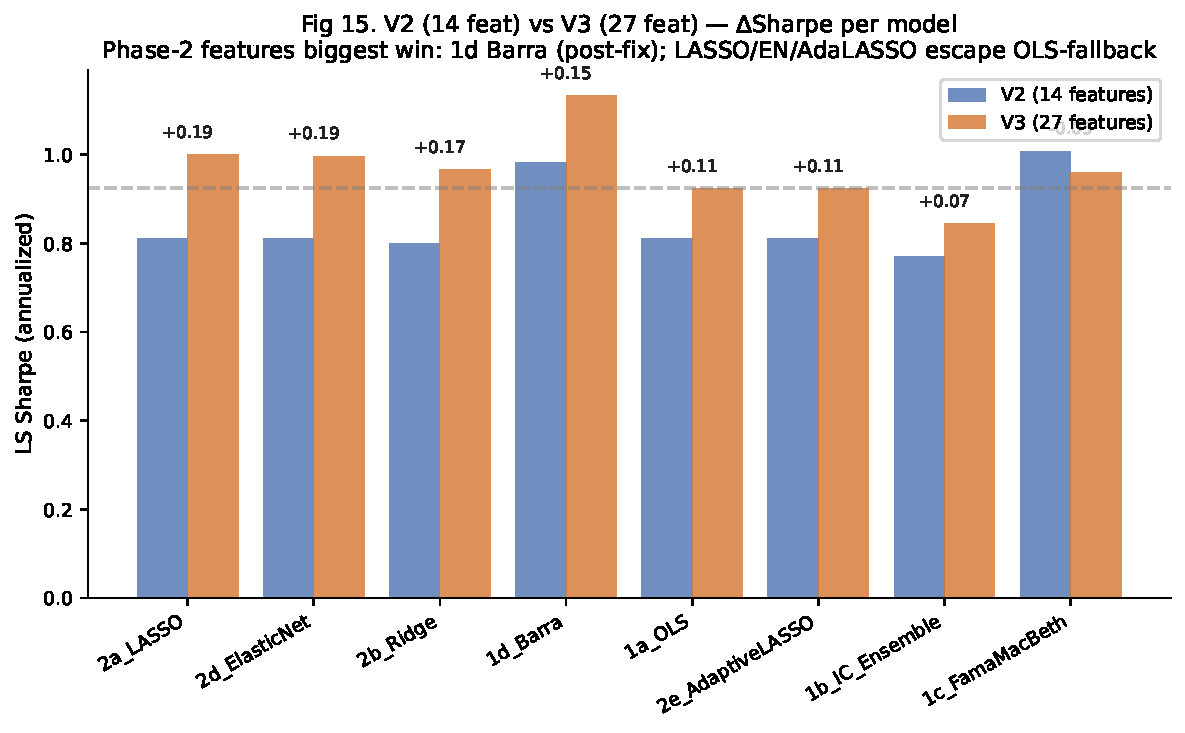
\includegraphics[width=0.85\textwidth]{fig_v2_vs_v3.pdf}
  \caption{Walk-forward LS Sharpe per model under V2 (14~features)
    vs.\ V3 (27~features). The Phase-2 feature expansion (IBES signals,
    Phase-2 firm-level signals, missingness flags) improves Sharpe for
    most models; Barra benefits most (0.982 $\to$ 1.134).}
  \label{fig:v2-vs-v3}
\end{figure}

\end{document}